%File: anonymous-submission-latex-2026.tex
\documentclass[letterpaper]{article} % DO NOT CHANGE THIS
\usepackage[submission]{aaai2026}  % DO NOT CHANGE THIS
\usepackage{times}  % DO NOT CHANGE THIS
\usepackage{helvet}  % DO NOT CHANGE THIS
\usepackage{courier}  % DO NOT CHANGE THIS
\usepackage[hyphens]{url}  % DO NOT CHANGE THIS
\usepackage{graphicx} % DO NOT CHANGE THIS
\urlstyle{rm} % DO NOT CHANGE THIS
\def\UrlFont{\rm}  % DO NOT CHANGE THIS
\usepackage{natbib}  % DO NOT CHANGE THIS AND DO NOT ADD ANY OPTIONS TO IT
\usepackage{caption} % DO NOT CHANGE THIS AND DO NOT ADD ANY OPTIONS TO IT
\frenchspacing  % DO NOT CHANGE THIS
\setlength{\pdfpagewidth}{8.5in} % DO NOT CHANGE THIS
\setlength{\pdfpageheight}{11in} % DO NOT CHANGE THIS
%
% These are recommended to typeset algorithms but not required. See the subsubsection on algorithms. Remove them if you don't have algorithms in your paper.
\usepackage{algorithm}
\usepackage{algorithmic}

% YipanWei Edited
\usepackage[table]{xcolor}
\usepackage{multirow}
\usepackage{arydshln}

\definecolor{DarkGreen}{RGB}{34,120,50}


\newcommand{\pub}[1]{{\color{gray}{\footnotesize{[{#1}]}}}}

\newcommand{\tworowbestreshl}[2]{%
\begin{tabular}{@{}c@{}}
{#1}  \\
{\small\color{DarkGreen}{$+$ \textbf{#2}}}
\end{tabular}%
}

%
% These are are recommended to typeset listings but not required. See the subsubsection on listing. Remove this block if you don't have listings in your paper.
\usepackage{newfloat}
\usepackage{listings}
\DeclareCaptionStyle{ruled}{labelfont=normalfont,labelsep=colon,strut=off} % DO NOT CHANGE THIS
\lstset{%
	basicstyle={\footnotesize\ttfamily},% footnotesize acceptable for monospace
	numbers=left,numberstyle=\footnotesize,xleftmargin=2em,% show line numbers, remove this entire line if you don't want the numbers.
	aboveskip=0pt,belowskip=0pt,%
	showstringspaces=false,tabsize=2,breaklines=true}
\floatstyle{ruled}
\newfloat{listing}{tb}{lst}{}
\floatname{listing}{Listing}
%
% Keep the \pdfinfo as shown here. There's no need
% for you to add the /Title and /Author tags.
\pdfinfo{
/TemplateVersion (2026.1)
}
\definecolor{LAMPYellow}{RGB}{255,220,112}
\definecolor{HeaderGray}{RGB}{235,235,235}
\definecolor{AvgBlue}{RGB}{226,241,255}
\definecolor{GainGreen}{RGB}{32,132,84}
\definecolor{DropRed}{RGB}{190,54,54}
\newcommand{\tblhead}[1]{\strut #1}
\newcommand{\lampcell}[1]{\begingroup\setlength{\fboxsep}{0pt}\colorbox{LAMPYellow}{\makebox[6.7em][c]{\rule[-1.12ex]{0pt}{4.45ex}\bfseries\boldmath #1}}\endgroup}
\newcommand{\avgcell}[1]{\begingroup\def\avgcontent{#1}\def\avgheader{Avg}\ifx\avgcontent\avgheader\bfseries #1\else\setlength{\fboxsep}{0pt}\colorbox{AvgBlue}{\makebox[3.55em][c]{\strut #1}}\fi\endgroup}
\newcommand{\metriclampcell}[1]{\begingroup\setlength{\fboxsep}{0pt}\colorbox{LAMPYellow}{\makebox[7.05em][c]{\rule[-0.96ex]{0pt}{3.95ex}\bfseries\boldmath #1}}\endgroup}
\newcommand{\lampband}{\noalign{\begingroup\color{LAMPYellow}\hrule height 3.35ex\endgroup\kern-3.35ex}}
\newcommand{\headband}{\noalign{\begingroup\color{HeaderGray}\hrule height 6.15ex\endgroup\kern-6.15ex}}
\newcommand{\gainup}[1]{\makebox[5.85em][l]{\textcolor{DropRed}{\(\uparrow\)#1}}}
\newcommand{\gaindown}[1]{\makebox[5.85em][l]{\textcolor{DropRed}{\(\downarrow\)#1}}}
\newcommand{\dropdown}[1]{\makebox[5.85em][l]{\textcolor{DropRed}{\(\downarrow\)#1}}}
\newcommand{\neutraldelta}[1]{\makebox[5.85em][l]{\textcolor{GainGreen}{#1}}}
\newcommand{\compactdrop}[1]{\textcolor{DropRed}{\(\downarrow\)#1}}
\newcommand{\compactgain}[1]{\textcolor{DropRed}{\(\uparrow\)#1}}
\newcommand{\compactneutral}[1]{\textcolor{GainGreen}{#1}}

% DISALLOWED PACKAGES
% \usepackage{authblk} -- This package is specifically forbidden
% \usepackage{balance} -- This package is specifically forbidden
% \usepackage{color (if used in text)
% \usepackage{CJK} -- This package is specifically forbidden
% \usepackage{float} -- This package is specifically forbidden
% \usepackage{flushend} -- This package is specifically forbidden
% \usepackage{fontenc} -- This package is specifically forbidden
% \usepackage{fullpage} -- This package is specifically forbidden
% \usepackage{geometry} -- This package is specifically forbidden
% \usepackage{grffile} -- This package is specifically forbidden
% \usepackage{hyperref} -- This package is specifically forbidden
% \usepackage{navigator} -- This package is specifically forbidden
% (or any other package that embeds links such as navigator or hyperref)
% \indentfirst} -- This package is specifically forbidden
% \layout} -- This package is specifically forbidden
% \multicol} -- This package is specifically forbidden
% \nameref} -- This package is specifically forbidden
% \usepackage{savetrees} -- This package is specifically forbidden
% \usepackage{setspace} -- This package is specifically forbidden
% \usepackage{stfloats} -- This package is specifically forbidden
% \usepackage{tabu} -- This package is specifically forbidden
% \usepackage{titlesec} -- This package is specifically forbidden
% \usepackage{tocbibind} -- This package is specifically forbidden
% \usepackage{ulem} -- This package is specifically forbidden
% \usepackage{wrapfig} -- This package is specifically forbidden
% DISALLOWED COMMANDS
% \nocopyright -- Your paper will not be published if you use this command
% \addtolength -- This command may not be used
% \balance -- This command may not be used
% \baselinestretch -- Your paper will not be published if you use this command
% \clearpage -- No page breaks of any kind may be used for the final version of your paper
% \columnsep -- This command may not be used
% \newpage -- No page breaks of any kind may be used for the final version of your paper
% \pagebreak -- No page breaks of any kind may be used for the final version of your paperr
% \pagestyle -- This command may not be used
% \tiny -- This is not an acceptable font size.
% \vspace{- -- No negative value may be used in proximity of a caption, figure, table, section, subsection, subsubsection, or reference
% \vskip{- -- No negative value may be used to alter spacing above or below a caption, figure, table, section, subsection, subsubsection, or reference

\setcounter{secnumdepth}{0} %May be changed to 1 or 2 if section numbers are desired.

% The file aaai2026.sty is the style file for AAAI Press
% proceedings, working notes, and technical reports.
%

% Title

% Your title must be in mixed case, not sentence case.
% That means all verbs (including short verbs like be, is, using,and go),
% nouns, adverbs, adjectives should be capitalized, including both words in hyphenated terms, while
% articles, conjunctions, and prepositions are lower case unless they
% directly follow a colon or long dash

% LAMP-Merge：面向单次异步临床模型的长尾感知医学原型融合。
\title{LAMP-Merge: Long-tail-Aware Medical Prototype Merging for One-shot Asynchronous Clinical Models}
\author{
    %Authors
    % All authors must be in the same font size and format.
    Written by AAAI Press Staff\textsuperscript{\rm 1}\thanks{With help from the AAAI Publications Committee.}\\
    AAAI Style Contributions by Pater Patel Schneider,
    Sunil Issar,\\
    J. Scott Penberthy,
    George Ferguson,
    Hans Guesgen,
    Francisco Cruz\equalcontrib,
    Marc Pujol-Gonzalez\equalcontrib
}
\affiliations{
    %Afiliations
    \textsuperscript{\rm 1}Association for the Advancement of Artificial Intelligence\\
    % If you have multiple authors and multiple affiliations
    % use superscripts in text and roman font to identify them.
    % For example,

    % Sunil Issar\textsuperscript{\rm 2},
    % J. Scott Penberthy\textsuperscript{\rm 3},
    % George Ferguson\textsuperscript{\rm 4},
    % Hans Guesgen\textsuperscript{\rm 5}
    % Note that the comma should be placed after the superscript

    1101 Pennsylvania Ave, NW Suite 300\\
    Washington, DC 20004 USA\\
    % email address must be in roman text type, not monospace or sans serif
    proceedings-questions@aaai.org
%
% See more examples next
}

%Example, Single Author, ->> remove \iffalse,\fi and place them surrounding AAAI title to use it
\iffalse
\title{My Publication Title --- Single Author}
\author {
    Author Name
}
\affiliations{
    Affiliation\\
    Affiliation Line 2\\
    name@example.com
}
\fi

\iffalse
%Example, Multiple Authors, ->> remove \iffalse,\fi and place them surrounding AAAI title to use it
\title{My Publication Title --- Multiple Authors}
\author {
    % Authors
    First Author Name\textsuperscript{\rm 1},
    Second Author Name\textsuperscript{\rm 2},
    Third Author Name\textsuperscript{\rm 1}
}
\affiliations {
    % Affiliations
    \textsuperscript{\rm 1}Affiliation 1\\
    \textsuperscript{\rm 2}Affiliation 2\\
    firstAuthor@affiliation1.com, secondAuthor@affilation2.com, thirdAuthor@affiliation1.com
}
\fi


% REMOVE THIS: bibentry
% This is only needed to show inline citations in the guidelines document. You should not need it and can safely delete it.
\usepackage{bibentry}
% END REMOVE bibentry

\begin{document}

\maketitle

\begin{abstract}
%
% 多中心医学模型通常处于异步医院流程、异构成像设备以及不完整诊断标签覆盖的共同约束下。本文研究单次异步医学模型融合问题：每个客户端在本地训练完成后仅上传一次，服务器在不访问原始医学图像且不执行联邦优化轮次的条件下构建全局模型。我们指出，将通用模型融合直接迁移到该场景会破坏一个关键假设：每个本地检查点并不是全局诊断空间的完整副本，而是由本地可见疾病支撑的局部专家。该错配会导致聚合诱导的预测坍缩，即融合模型把预测集中到少数主导类别。更隐蔽的是，医学长尾患病率会使这种坍缩在原始准确率上呈现出具有迷惑性的竞争力。为解决上述问题，本文提出 LAMP-Merge，一种长尾感知医学原型融合框架，将融合目标从全局参数插值转向类别级诊断证据重建。LAMP-Merge 利用客户端侧类别统计构建诊断原型头，并用有界先验偏置校准疾病患病率。在五个医学数据集、四类视觉模型、三种客户端数量和三种非独立同分布偏斜水平上，LAMP-Merge 在 60 个客户端平均单元中的 57 个单元达到或超过最强非 LAMP 基线，同时提升平衡准确率、宏 F1 和预测坍缩诊断指标。
Multicenter medical models are commonly trained under asynchronous hospital workflows, heterogeneous acquisition devices, and incomplete diagnostic-label coverage. We study single-shot asynchronous medical model merging, where each client uploads only once after local training and the server constructs a global model without accessing raw medical images or performing federated optimization rounds. We argue that directly transferring general-purpose model merging to this setting breaks a key assumption: each local checkpoint is not a complete view of the global diagnostic space, but a partial expert supported by locally observed diseases. This mismatch leads to aggregation-induced prediction collapse, where the merged model concentrates predictions on a few dominant classes. More subtly, long-tailed medical prevalence can make such collapse deceptively competitive under raw accuracy. To address these issues, we propose LAMP-Merge, a long-tail-aware medical prototype-merging framework that shifts the merge target from global parameter interpolation to class-level diagnostic-evidence reconstruction. LAMP-Merge builds a diagnostic prototype head from client-side class statistics and calibrates disease prevalence with a bounded prior bias. Across five medical datasets, four vision-model families, three client-population sizes, and three non-IID skew levels, LAMP-Merge matches or surpasses the strongest non-LAMP baseline in 57 of 60 client-averaged settings, while improving balanced accuracy, macro-F1, and prediction-collapse diagnostics.

%医学模型融合 异步融合 预测性坍缩 长尾校准 隐私保护学习
Index Terms:medical model merging, asynchronous fusion, predictive collapse, long-tail calibration, privacy-preserving learning
\end{abstract}


% Uncomment the following to link to your code, datasets, an extended version or similar.
% You must keep this block between (not within) the abstract and the main body of the paper.
% \begin{links}
%     \link{Code}{https://aaai.org/example/code}
%     \link{Datasets}{https://aaai.org/example/datasets}
%     \link{Extended version}{https://aaai.org/example/extended-version}
% \end{links}

\section{Introduction}

% 联邦学习和模型融合为隐私敏感的多中心医学智能提供了两条重要协作路径。联邦学习允许医院在不共享原始数据的情况下进行协同训练，模型融合则进一步降低通信和训练成本，使已经独立训练完成的本地模型能够在训练后被整合为一个统一模型。这两类方法对于医学影像尤其有吸引力：一方面，单个医院通常难以覆盖完整疾病谱、罕见病例和多样化成像条件；另一方面，隐私法规、设备差异和院内流程使原始医学影像集中化难以实现。因此，若能在不暴露原始数据的前提下整合多中心知识，将为真实临床部署提供一种高效且可行的协作机制。
Federated learning~\cite{pmlr-v54-mcmahan17a,li2020fedprox,karimireddy2020scaffold,kairouz2021advances} and model merging~\cite{izmailov2018averaging,pmlr-v162-wortsman22a,ilharco2023editingmodelstaskarithmetic,yadav2023tiesmergingresolvinginterferencemerging} provide two important collaboration routes for privacy-sensitive multicenter medical intelligence. Federated learning enables hospitals to train collaboratively without sharing raw data~\cite{sheller2020federated,rieke2020future}, while model merging further reduces communication and optimization costs by integrating independently trained local models after training~\cite{ainsworth2023gitrebasinmergingmodels,stoica2024zipit,matena2022mergingmodelsfisherweightedaveraging}. These paradigms are particularly attractive for medical imaging: a single hospital rarely covers the full disease spectrum, rare cases, and diverse acquisition conditions, whereas privacy regulations, device heterogeneity, and institutional workflows make centralized raw-image collection impractical~\cite{kaissis2020secure,bonawitz2019towards,abadi2016deep}. Therefore, integrating multicenter knowledge without exposing raw data is a practical and efficient route toward real clinical deployment.

% 尽管模型融合和联邦学习相关范式在自然图像和通用视觉任务中取得了成功，将其迁移到医学数据仍然面临挑战。关键在于，通用模型融合通常隐含假设不同客户端检查点包含相对完整且可比较的全局判别结构，即各本地模型可以在参数空间、任务向量空间或更新方向上直接对齐。然而，该范式在医学场景中并不成立。医疗中心之间不仅存在设备域偏移，还存在诊断类别可及性差异：某些中心可能只覆盖常见病或特定检查类型，而缺乏罕见疾病样本。由此得到的本地模型不是全局任务的完整副本，而是由本地可见疾病支撑的局部诊断专家。
Despite their success on natural images and general visual tasks~\cite{izmailov2018averaging,pmlr-v162-wortsman22a,ilharco2023editingmodelstaskarithmetic,entezari2022role,ainsworth2023gitrebasinmergingmodels}, transferring these paradigms to medical data remains challenging. A key reason is that general-purpose model merging implicitly assumes that different client checkpoints contain relatively complete and comparable global discriminative structures; local models are expected to align through parameter space, task-vector space, update signs, or curvature statistics~\cite{yadav2023tiesmergingresolvinginterferencemerging,yu2024languagemodelssupermario,matena2022mergingmodelsfisherweightedaveraging,jin2025datalessknowledgefusionmerging}. This assumption does not hold in medical scenarios. Medical centers differ not only in device domains but also in diagnostic-class availability: some centers may mainly cover common diseases or specific examination types, while having few rare-disease samples~\cite{9557808,10.1371/journal.pmed.1002683,li2021fedbn}. The resulting local models are not complete replicas of the global task, but partial diagnostic experts supported by locally observed diseases.

% 如图 1 所示，我们将这些挑战归纳为医学模型融合中的两种诊断结构异常特征。
As illustrated in Fig.~\ref{fig:intro-collapse}, we summarize these challenges as two diagnostic-structure abnormalities in medical model merging:
\begin{itemize}
    \item \textbf{Intra-client: limited local diagnostic coverage.} Each client has reliable supervision only for observed classes; thus, a local model may be locally discriminative but still lack evidence for the full global diagnostic space~\cite{9557808,li2021fedbn}.
    \item \textbf{Inter-client: aggregation-induced prediction collapse.} Inconsistent class coverage and long-tailed prevalence can cause generic merging methods to mix reliable, absent, and conflicting class directions, making the merged global model concentrate predictions on a few dominant classes. More subtly, long-tailed medical distributions can make such collapse appear competitive under raw accuracy, thereby hiding insufficient global diagnostic discrimination~\cite{BUDA2018249,5597285}.
\end{itemize}

\begin{figure}[t]
    \centering
    
\includegraphics[width=0.96\linewidth]{figures/intro.png}
    \caption{In multicenter healthcare settings, individual clients typically observe only a subset of the global diagnostic space. Conventional parameter-level model-merging methods can therefore cause the merged global model’s predictions to concentrate on a small number of dominant classes.}
    \label{fig:intro-collapse}
\end{figure}

% 为解决这些问题，我们提出 LAMP-Merge，一种面向单次异步医学图像模型融合的长尾感知医学原型融合方法。该方法将融合目标从全局参数插值转变为类别级诊断证据重建。其核心思想是使用客户端上传的类别级统计作为全局诊断空间的同步信号，在不访问原始医学图像、不使用服务器端验证集且不进行多轮联邦通信的条件下重建全局诊断分类器。具体而言，LAMP-Merge 包含两个关键机制：诊断原型重建利用共享参考特征空间中的类别原型聚合可靠的类别级证据；长尾患病率校准利用客户端上传的类别计数引入有界先验偏置，从而在缓解预测坍缩的同时保留具有临床意义的多数类患病率。
To address these issues, we propose \textbf{LAMP-Merge}, a long-tail-aware medical prototype-merging method for single-shot asynchronous medical image model merging. LAMP-Merge shifts the merge target from global parameter interpolation to class-level diagnostic-evidence reconstruction. The key idea is to use client-uploaded class-level statistics as a synchronization signal for the global diagnostic space, allowing the server to reconstruct a global diagnostic classifier without accessing raw medical images, using a server-side validation set, or conducting multi-round federated communication. Specifically, LAMP-Merge consists of two mechanisms: diagnostic prototype reconstruction aggregates reliable class-level evidence through prototypes in a shared reference feature space, and long-tail prevalence calibration injects a bounded prior bias from client-uploaded class counts, thereby mitigating prediction collapse while preserving clinically meaningful majority-class prevalence.

\begin{figure*}[t]
    \centering
    
\includegraphics[width=0.92\textwidth,height=0.34\textheight]{figures/method.png}
    \caption{Local models from multicenter hospitals typically contain only partial diagnostic knowledge, while raw medical images cannot be centrally shared. LAMP-Merge reconstructs a privacy-friendly global medical classifier through diagnostic prototype reconstruction and long-tail prevalence calibration, without accessing raw data or requiring multi-round federated optimization.}
    \label{fig_method}
\end{figure*}

% 我们的主要贡献总结如下：
Our main contributions are summarized as follows:
\begin{itemize}
    \item \textbf{Medical Merging Diagnosis.} We revisit model merging under single-shot asynchronous medical collaboration and identify limited local diagnostic coverage and aggregation-induced prediction collapse as two key abnormalities caused by medical class availability and long-tailed prevalence.
    \item \textbf{LAMP-Merge.} We propose a long-tail-aware medical prototype-merging method that reconstructs a global diagnostic classifier from client-side class prototypes and prevalence statistics without exposing raw images or requiring multi-round federated optimization.
    \item \textbf{Empirical Validation.} We conduct full-scope experiments on five medical image datasets, four vision-model families, three client-population sizes, and three non-IID skew levels, showing that LAMP-Merge consistently outperforms strong model-merging baselines and improves prediction-collapse diagnostics.
\end{itemize}

\section{Related Works}

\subsection{Model Merging}

% 模型融合方法通常在参数空间、任务向量空间或几何空间中整合独立训练的检查点。权重平均和 Model Soups 直接插值参数；置换感知匹配对齐隐藏单元对称性；ZipIt 执行特征级拼接；Task Arithmetic、TIES-Merging 和 DARE 操作任务增量与符号冲突；Fisher、RegMean、Model Stock、Breadcrumbs、Iso-C、FreeMerge 与 RobustMerge 进一步引入曲率、均值统计、子空间、频域或鲁棒性假设。然而，这些方法共享一种类别无关的融合接口：其变量是全局参数、任务向量、更新符号或几何统计，而不是类别级诊断证据。它们无法表达某个客户端是否对某个医学类别具有可靠监督。在局部类别覆盖不完整且患病率长尾的场景中，可靠类别方向会与其他客户端的缺失或冲突方向混合，从而产生聚合诱导的预测坍缩。
Model-merging methods integrate independently trained checkpoints in parameter, task-vector, or geometric spaces. Weight averaging~\cite{izmailov2018averaging} and Model Soups~\cite{pmlr-v162-wortsman22a} directly interpolate parameters; permutation-aware matching~\cite{entezari2022role,ainsworth2023gitrebasinmergingmodels} aligns hidden-unit symmetries; ZipIt~\cite{stoica2024zipit} performs feature-level zipping; Task Arithmetic~\cite{ilharco2023editingmodelstaskarithmetic}, TIES-Merging~\cite{yadav2023tiesmergingresolvinginterferencemerging}, and DARE~\cite{yu2024languagemodelssupermario} manipulate task deltas and sign conflicts; Fisher merging~\cite{matena2022mergingmodelsfisherweightedaveraging}, RegMean~\cite{jin2025datalessknowledgefusionmerging}, Model Stock~\cite{jang2025modelstockneedjust}, Breadcrumbs~\cite{davari2024modelbreadcrumbsscalingmultitask}, Iso-C~\cite{marczak2025taskleftbehindisotropic}, FreeMerge~\cite{zheng2025freemergingfouriertransformefficient}, and RobustMerge~\cite{zeng2025robustmergeparameterefficientmodelmerging} introduce curvature, mean-statistic, subspace, frequency-domain, or robustness assumptions.

However, these methods share a class-agnostic merging interface: their variables are global parameters, task vectors, update signs, or geometric statistics rather than class-level diagnostic evidence. \textbf{They do not encode whether a client has reliable supervision for a specific medical class.} Under incomplete local class coverage and long-tailed prevalence, reliable class directions can be mixed with absent or conflicting directions from other clients, resulting in aggregation-induced prediction collapse\cite{BUDA2018249,10.1371/journal.pmed.1002683}.

\subsection{Medical Model Merging}

% 医学融合研究通常利用医学数据的领域结构，例如非规则临床时间序列、生理传感器图结构和影像-电子病历融合。mTAN、Raindrop 和 MedFuse 表明，医学任务受益于对临床采样机制、模态异质性和患者级时间关系的建模。然而，这些方法的融合对象通常是患者级输入、多模态记录或临床表征，而不是独立训练完成的图像分类器检查点。它们往往需要患者样本、时间戳、电子病历或服务器端验证反馈，这与常见隐私约束冲突。MedMerge 是相关的训练自由医学知识迁移框架，但目标是医学视觉语言模型的跨模态适配，而不是同一分类任务下的异步检查点融合。因此，现有医学融合路线与本文的隐私约束和单次上传协议并不匹配。LAMP-Merge 仅使用本地计算的类别原型和患病率计数，使医学结构以可上传的形式参与融合。
Medical fusion studies exploit domain structures such as irregular clinical time series, physiological sensor graphs, and image-EHR fusion. mTAN~\cite{shukla2021multitimeattentionnetworksirregularly}, Raindrop~\cite{zhang2022graphguidednetworkirregularlysampled}, and MedFuse~\cite{hayat2023medfusemultimodalfusionclinical} show that medical tasks benefit from modeling clinical sampling mechanisms, modality heterogeneity, and patient-level temporal relations.

However, their fusion objects are usually patient-level inputs, multimodal records, or clinical representations rather than independently trained image-classifier checkpoints. They often require patient samples, timestamps, electronic health records, or server-side validation feedback, which conflicts with common privacy constraints~\cite{kaissis2020secure,sheller2020federated,bonawitz2019towards}. MedMerge~\cite{11382027} is a relevant training-free medical knowledge-transfer framework, but it targets cross-modal adaptation for medical vision-language models rather than asynchronous checkpoint merging for the same classification task. \textbf{Thus, existing medical fusion routes are mismatched with our privacy and single-upload protocol constraints.} LAMP-Merge keeps the medical structure uploadable by using only locally computed class prototypes and prevalence counts.

\subsection{Federated Learning}

% 联邦学习和去中心化学习通过通信协议完成协作训练。FedAvg 及其变体或医学部署依赖多轮服务器-客户端更新；Swarm Learning 和 Gossip Learning 减弱中心化角色，但仍要求参与者持续训练、交换模型并从中间状态继续优化。然而，本文场景发生在本地训练完成之后：医院可能无法长期在线、反复接收全局检查点或执行额外优化轮次。因此，瓶颈不仅是隐私，也是通信可实现性。LAMP-Merge 仅需要本地模型接口和类别级统计的一次上传，使服务器无需多轮反馈即可构建统一诊断模型。
Federated and decentralized learning perform collaborative training through communication protocols. FedAvg~\cite{pmlr-v54-mcmahan17a} and its variants or medical deployments~\cite{li2020fedprox,karimireddy2020scaffold,li2021fedbn,kaissis_secure_2020,sheller2020federated,rieke2020future,kairouz2021advances} rely on repeated server-client updates; Swarm Learning~\cite{warnat-herresthal_swarm_2021} and Gossip Learning~\cite{hegedhus_gossip_2019} reduce centralization but still require participants to continue training, exchanging models, and optimizing from intermediate states.

However, our setting begins after local training has finished. Hospitals may not remain online, receive global checkpoints repeatedly, or run additional optimization rounds. \textbf{The bottleneck is therefore communication feasibility in addition to privacy.} LAMP-Merge requires one upload of a local model interface and class-level statistics, enabling the server to construct a unified diagnostic model without a multi-round feedback loop.

\section{Method}

% 在本节中，我们首先正式描述单次异步医学模型融合的任务设定，并刻画通用模型融合应用于医学数据时暴露出的诊断结构病理现象，即局部诊断覆盖受限与聚合诱导预测坍缩。为校正这些内在失配，我们提出 LAMP-Merge，一个由诊断原型重建和长尾患病率校准两阶段组成的框架，如图所示。
In this section, we first formulate the single-shot asynchronous medical model-merging problem and characterize the diagnostic-structure pathologies exposed when generic model merging is applied to medical data, namely limited local diagnostic coverage and aggregation-induced prediction collapse. To correct these intrinsic mismatches, we propose \textbf{LAMP-Merge}, a two-stage framework composed of diagnostic prototype reconstruction and long-tail prevalence calibration, as shown in Fig.~\ref{fig_method}.

\subsection{Preliminaries}

\subsubsection{Problem Formulation.}

% 假设存在 K 个医学客户端。客户端 i 持有私有标注数据集 D_i={(x,y)}，其来自覆盖 C 个诊断类别的类别偏斜医学分布。令 D_i,c 表示客户端 i 中属于诊断类别 c 的样本子集。在医学划分中，D_i,c 对许多类别可能为空，因此客户端 i 只对其已见类别具有可靠监督。目标是在这些条件下构建一个全局诊断模型。
Assume $K$ medical clients. Client $i$ owns a private labeled dataset $D_i=\{(x,y)\}$ drawn from a class-skewed medical distribution over $C$ diagnosis classes. Let $D_{i,c}$ denote the subset of client $i$ belonging to diagnosis class $c$. In medical partitions, $D_{i,c}$ can be empty for many classes; therefore, client $i$ has reliable supervision only for its observed classes. The goal is to construct a global diagnostic model under this partial and heterogeneous diagnostic-label coverage.

\subsubsection{Upload and Server Constraints.}

% 本文研究单次异步融合：每个客户端在本地训练后仅上传一次，服务器不能访问原始医学图像、逐样本特征、逐样本预测或服务器端验证集，也不向客户端发起多轮更新。客户端允许上传类别级统计量。具体而言，n_i,c 表示类别支持数，m_i,c 表示类别患病率计数，mu_i,c 表示在共享参考特征空间中计算得到的类别原型。服务器仅利用本地检查点接口和这些类别级统计执行一次融合。该问题不同于联邦学习，因为客户端不会根据服务器反馈继续优化；也不同于标准模型融合，因为类别证据是否存在本身成为融合变量。
We study single-shot asynchronous merging: after local training, each client uploads only once, while the server cannot access raw medical images, per-sample features, per-sample predictions, or a server-side validation set, and does not issue multi-round updates to clients. Clients are allowed to upload class-level statistics. Specifically, $n_{i,c}$ denotes the class-support count, $m_{i,c}$ denotes the class-prevalence count, and $\mu_{i,c}$ denotes the class prototype computed in a shared reference feature space. The server performs one merge using only the local checkpoint interfaces and these class-level statistics. This setting differs from federated learning because clients do not continue optimization from server feedback; it also differs from standard model merging because the presence of class-level diagnostic evidence becomes an explicit merging variable.

\subsection{Motivation}

% 尽管通用模型融合具有训练成本低和参数效率高的优势，但我们发现其诊断结构在医学模型融合中会严重退化。我们通过预测分布诊断和患病率分析揭示了两种关键异常现象。
Although generic model merging is training-free and parameter-efficient, we find that its diagnostic structure can severely degenerate in medical model merging. Prediction-distribution diagnosis and prevalence analysis reveal two key abnormalities:
\begin{itemize}
    \item \textbf{Aggregation-induced prediction collapse.} Under partial diagnostic coverage, parameter-level merging can turn several locally useful predictors into a globally collapsed predictor. The merged model tends to allocate most test images to a few dominant classes, indicating that global class-discriminative structure has not been reconstructed.
    \item \textbf{Prevalence prior cannot be ignored.} Medical datasets often exhibit clinically meaningful long-tailed prevalence. Therefore, completely suppressing majority-class dominance is also inappropriate: a collapsed predictor is undesirable, but a merger should still preserve calibrated disease prevalence when the dominant class reflects the true clinical prior.
\end{itemize}

% 上述现象分别对应 LAMP-Merge 的两个设计目标：首先通过诊断原型重建恢复多类别判别结构，其次通过长尾患病率校准保留真实类别先验。LAMP-Merge 因此将融合目标从参数空间共识转向诊断空间证据重建。
These observations correspond to the two design targets of LAMP-Merge: first, reconstructing multiclass discriminative structure through diagnostic prototypes; second, preserving the real class prior through long-tail prevalence calibration. LAMP-Merge therefore shifts the merge target from parameter-space consensus to diagnosis-space evidence reconstruction.

\subsection{Overview}

% LAMP-Merge 的核心框架如图所示。其核心思想是使用客户端类别级统计作为全局诊断空间的同步信号，将医学模型融合从全局参数平均转化为类别条件诊断证据重建，并辅以经过校准的类别先验信息。
The core framework of LAMP-Merge is illustrated in Fig.~\ref{fig_method}. The central idea is to use class-level client statistics as a synchronization signal for the global diagnostic space. This turns medical model merging from global parameter averaging into class-conditional diagnostic-evidence reconstruction, supplemented by calibrated class-prior information.

% 值得注意的是，LAMP-Merge 既不要求服务器访问客户端原始图像，也不依赖服务器端验证集、逐样本特征或逐样本预测。客户端仅上传类别级统计量，因此该框架保持单次异步边界，并区别于需要反复下发模型和本地再训练的联邦学习流程。
Notably, LAMP-Merge neither requires the server to access clients' raw images nor relies on a server-side validation set, per-sample features, or per-sample predictions. Clients upload only class-level statistics; thus, the framework preserves the single-shot asynchronous boundary and differs from federated learning procedures that repeatedly broadcast models and retrain locally.

% 该框架包含两个组件。第一个组件通过具有类别支持的原型重建多类别诊断方向，以抵消聚合诱导的坍缩。第二个组件注入有界长尾先验，避免重建步骤过度抹除具有临床意义的多数类患病率。
The framework contains two components. The first reconstructs multiclass diagnostic directions from class-supported prototypes, counteracting aggregation-induced collapse. The second injects a bounded long-tail prior, preventing the reconstruction step from overcorrecting clinically meaningful majority prevalence.

\subsection{Diagnostic Prototype Reconstruction Module}

% 为缓解由异构诊断覆盖和冲突类别证据带来的聚合后预测坍缩，诊断原型重建模块将融合目标从参数平均转化为类别条件证据重建。它不直接平均本地分类器，而是先在共享参考空间中收集每个客户端对每个诊断类别的可靠证据，再由服务器合成覆盖全局标签空间的诊断头。
To mitigate the \textbf{post-aggregation prediction collapse} caused by heterogeneous diagnostic coverage and conflicting class evidence, the diagnostic prototype reconstruction module shifts the merging target from parameter averaging to class-conditional evidence reconstruction. Instead of directly averaging local classifiers, it first collects reliable evidence for each diagnosis class in a shared reference space and then synthesizes a global diagnostic head over the full label space.

\subsubsection{1) Reference-space Class Prototype Extraction.}

% 首先，所有客户端使用同一个冻结参考骨干网络提取类别原型。令 phi_0 表示本地训练前由共享模型配置实例化得到的参考骨干网络，T(.) 表示评估变换。对于每个诊断类别 c，客户端 i 在本地计算参考空间类别原型 mu_i,c，其中 n_i,c=|D_i,c| 是类别支持数。
First, all clients extract class prototypes with the same frozen reference backbone. Let $\phi_0$ be the reference backbone instantiated from the shared model configuration before local training, and let $T(\cdot)$ be the evaluation transform. For each diagnosis class $c$, client $i$ locally computes a reference-space class prototype
\begin{equation}
\mu_{i,c}=\frac{1}{n_{i,c}}\sum_{(x,y)\in D_i}\mathbf{1}[y=c]\phi_0(T(x)),
\end{equation}
where $n_{i,c}=|D_{i,c}|$ is the class support count. If $n_{i,c}=0$, the client uploads zero support for that class and contributes no prototype evidence.

\subsubsection{2) Support-aware Evidence Aggregation.}

% 其次，服务器将类别支持数转换为证据权重，以刻画客户端对该类别的可靠程度。gamma=0.45 为默认证据指数。该权重使具有更多同类监督样本的客户端对类别 c 贡献更大，同时完全排除未观察到该类别的客户端。
Second, the server converts class-support counts into evidence weights to characterize the reliability of each client for a given class:
\begin{equation}
e_{i,c}=(n_{i,c}+1)^\gamma \mathbf{1}[n_{i,c}>0],
\end{equation}
where $\gamma=0.45$ is the default evidence exponent. This weight gives larger class-specific contribution to clients with more supervised samples of class $c$, while excluding clients that never observe this class. The normalized reliability is
\begin{equation}
\alpha_{i,c}=\frac{e_{i,c}}{\sum_{j=1}^{K} e_{j,c}}.
\end{equation}

% 因此，全局诊断原型由各客户端原型按照类别可靠性加权得到。该步骤使服务器只聚合真正见过该类别的客户端证据，从而避免未见类别客户端的分类器方向稀释有效诊断信号。
The global diagnosis prototype is obtained by class-wise reliability-weighted aggregation:
\begin{equation}
p_c=\sum_{i=1}^{K}\alpha_{i,c}\mu_{i,c}.
\end{equation}
This step aggregates evidence only from clients that have actually observed class $c$, preventing absent-class classifiers from diluting valid diagnostic signals.

\subsubsection{3) Prototype-induced Diagnostic Head.}

% 最后，LAMP-Merge 将全局诊断原型映射为余弦原型分类器，其中 s=20 为默认分类头缩放因子。由此得到的分类头不是本地 head 的参数平均，而是由共享参考空间中的类别证据诱导得到，因此能够恢复覆盖全局诊断空间的多类别判别方向。
Finally, LAMP-Merge maps global diagnosis prototypes into a cosine prototype classifier:
\begin{equation}
w_c=s\frac{p_c}{\|p_c\|_2},
\end{equation}
where $s=20$ is the default head scale. The resulting head is not an average of local classifier parameters; it is induced by class evidence in the shared reference space, thereby restoring multiclass diagnostic directions over the global label space.

\subsection{Long-tail Prevalence Calibration}

% 为处理真实医学任务中长尾患病率不可忽略的问题，长尾患病率校准模块在原型重建之后引入一个有界类别先验。该模块并不把模型重新推向单类坍缩，而是在多类别诊断方向已经恢复的前提下，校准由客户端统计反映的临床患病率。
To address the fact that long-tailed prevalence cannot be ignored in real medical tasks, the long-tail prevalence calibration module introduces a bounded class prior after prototype reconstruction. This module does not push the model back to single-class collapse; instead, it calibrates the clinical prevalence reflected by client statistics after multiclass diagnostic directions have been restored.

\subsubsection{1) Client-reported Prevalence Prior.}

% 首先，每个客户端上传类别患病率计数 m_i,c。服务器据此估计全局类别先验 pi_c。该先验只来自类别级计数，而不是原始图像、逐样本特征或逐样本预测。
First, each client uploads class-prevalence counts $m_{i,c}$. The server estimates the global class prior
\begin{equation}
\pi_c=\frac{\sum_{i=1}^{K}m_{i,c}}{\sum_{k=1}^{C}\sum_{i=1}^{K}m_{i,k}}.
\end{equation}
This prior is computed only from class-level counts, not from raw images, per-sample features, or per-sample predictions.

\subsubsection{2) Long-tail Activation Criterion.}

% 其次，为避免在非长尾场景中过度校准，服务器用 r=C max_c pi_c 度量主导类别不平衡。该模块仅在 r>tau 时激活，其中 tau=2.5 为默认值。
Second, to avoid unnecessary calibration in non-long-tailed cases, the server measures dominant-class imbalance by
\begin{equation}
r=C\max_c \pi_c.
\end{equation}
The calibration module is activated only when $r>\tau$, where $\tau=2.5$ by default.

\subsubsection{3) Centered Log-prior Calibration.}

% 最后，当该模块被激活时，LAMP-Merge 构造中心化对数先验偏置 b_c，其默认最大校准强度为 lambda=5.0。中心化操作避免所有类别 logits 被整体平移，使该项只改变类别相对先验。
Finally, when the module is activated, LAMP-Merge constructs a centered log-prior bias
\begin{equation}
b_c=\lambda\left(\log\pi_c-\frac{1}{C}\sum_{k=1}^{C}\log\pi_k\right),
\end{equation}
with default maximum calibration strength $\lambda=5.0$. The centering term prevents a uniform shift of all class logits, so the bias only changes the relative class prior. This module calibrates prevalence without replacing the diagnostic directions reconstructed by the first module.

\subsection{Optimization Objective and Algorithm}

% LAMP-Merge 不在服务器端执行梯度优化。它的优化目标可以理解为构造一个同时满足两项要求的全局分类器：一方面，分类头 w_c 应来自类别支持的诊断原型；另一方面，输出 logits 应包含有界长尾先验。对于测试图像 x，最终类别得分为：
LAMP-Merge does not perform gradient-based optimization on the server. Its objective is to construct a global classifier that satisfies two requirements: the classifier head $w_c$ should be induced by class-supported diagnostic prototypes, and the output logits should include a bounded long-tail prior when prevalence imbalance is present. For a test image $x$, the final class score is
\begin{equation}
\ell_c(x)=w_c^\top\phi_0(T(x))+\mathbf{1}[r>\tau]\,b_c.
\end{equation}

% 最终预测由最大得分类别给出：
The final prediction is given by
\begin{equation}
\hat{y}(x)=\arg\max_{c\in\{1,\ldots,C\}}\ell_c(x).
\end{equation}

% 因此，完整算法可以概括为：客户端本地计算并上传类别支持数、参考空间类别原型和患病率计数；服务器先通过诊断原型重建得到 w_c，再通过长尾患病率校准得到 b_c，最后用上述得分函数执行推理。整个过程只需要一次客户端上传，不依赖服务器端验证数据或多轮客户端通信。
Thus, the complete algorithm proceeds as follows: clients locally compute and upload class-support counts, reference-space class prototypes, and prevalence counts; the server first obtains $w_c$ through diagnostic prototype reconstruction, then obtains $b_c$ through long-tail prevalence calibration, and finally performs inference using the score above. The whole procedure requires only one client upload and does not rely on server-side validation data or multi-round client communication.

\section{Experiments}

\subsection{Experimental Settings}

\subsubsection{1) Evaluation Datasets:}

We evaluate the merged models on five representative MedMNIST v2 benchmarks\cite{yang2023medmnist}: Blood, Derma, Organ-C, Organ-S, and Ultrasound. They cover blood-cell microscopy, dermoscopy, abdominal CT, and ultrasound image classification (detailed dataset descriptions are provided in the Appendix).

\subsubsection{2) Baselines:}

% 对比方法覆盖当前模型融合中的主要技术路线，包括参数平均、任务向量修剪、符号冲突处理、曲率或均值校正、模型库存、子空间各向同性融合、频域融合和鲁棒方向融合。这些方法构成通用模型融合的强基线，但其共同限制在于不显式建模医学类别证据。
We compare LAMP-Merge with twelve model-merging baselines covering the main technical routes of current model merging: \texttt{avg}\cite{pmlr-v162-wortsman22a}, \texttt{ties}\cite{yadav2023tiesmergingresolvinginterferencemerging}, \texttt{dare\_linear}\cite{yu2024languagemodelssupermario}, \texttt{dare\_ties}\cite{yu2024languagemodelssupermario}, \texttt{regmean}\cite{jin2025datalessknowledgefusionmerging}, \texttt{fisher}\cite{matena2022mergingmodelsfisherweightedaveraging}, \texttt{breadcrumbs}\cite{davari2024modelbreadcrumbsscalingmultitask}, \texttt{model\_stock}\cite{jang2025modelstockneedjust}, \texttt{from}\cite{ilharco2023editingmodelstaskarithmetic}, \texttt{iso\_c}\cite{marczak2025taskleftbehindisotropic}, \texttt{free\_merge}\cite{zheng2025freemergingfouriertransformefficient}, and \texttt{robustmerge}\cite{zeng2025robustmergeparameterefficientmodelmerging}. These baselines include weight averaging, task-vector pruning, sign-conflict resolution, curvature or mean-statistic correction, stock-style model interpolation, isotropic subspace merging, Fourier-domain fusion, and direction-robust merging.

\subsubsection{3) Merging Settings:}

% 实验遵循单次异步模型融合流程。每个客户端先在自己的医学图像数据上独立训练本地模型，并在本地计算 LAMP-Merge 所需的类别级统计，包括类别支持数、参考空间类别原型和类别患病率计数。这些统计与本地检查点接口一起只上传一次。随后服务器仅根据上传的检查点和类别级统计执行一次融合，并在全局测试集上评估融合模型。
Experiments follow a single-shot asynchronous model-merging protocol. Each client independently trains a local model on its own medical imaging data and then computes the class-level statistics required by LAMP-Merge locally, including class-support counts, reference-space class prototypes, and class-prevalence counts. These statistics are uploaded once together with an interface to the local checkpoint. The server performs a single model-merging step using only the uploaded checkpoints and class-level statistics, and evaluates the resulting merged model on a global test set.

% 我们评估四类基础视觉模型：ResNet、ConvNeXt、ViT-Tiny 和 Swin-Tiny。对于每个数据集-模型组合，我们构造非独立同分布客户端划分，客户端数量 K 属于 {3,5,7}，Dirichlet 偏斜参数 beta 属于 {0,0.01,0.1}，随机种子固定为 42。客户端平均结果先固定数据集、模型和 K，再对三个 beta 值求平均。
We evaluate four vision-model families: ResNet, ConvNeXt, ViT-Tiny, and Swin-Tiny\cite{he2016deep,liu2022convnet,dosovitskiy2021image,liu2021swin}. For each dataset-model pair, we construct non-IID client partitions with $K\in\{3,5,7\}$ clients and Dirichlet skew parameter $\beta\in\{0,0.01,0.1\}$, using seed 42\cite{hsu2019measuringeffectsnonidenticaldata}. A client-average result fixes the dataset, model, and $K$, and then averages over the three $\beta$ values.

\subsubsection{4) Implementation Environment:}

% 所有实验运行在配备两颗 Intel Xeon Silver 4210 CPU、四张 NVIDIA GeForce RTX 2080 Ti GPU 的服务器上；软件环境为 conda 环境 MM，使用 Python 3.10.20、PyTorch 2.6.0+cu118 和 CUDA runtime 11.8。
All experiments were run on a server with two Intel(R) Xeon(R) Silver 4210 CPUs, four NVIDIA GeForce RTX 2080 Ti GPUs, and the conda environment \texttt{MM} with Python 3.10.20, PyTorch 2.6.0+\texttt{cu118}, and CUDA runtime 11.8.

\subsection{Comparison With the State of the Arts}
% 主比较采用客户端平均准确率：对于每个固定的数据集、模型和客户端数量，先对三个 beta 偏斜水平求平均，再比较不同融合方法。若 LAMP-Merge 在某个单元中大于或等于最强非 LAMP 基线，则该单元计为成功。该设置检验方法是否在不同医学模态、骨干网络和客户端规模下稳定有效，而非只在单一划分上偶然胜出。
The main comparison uses client-average ACC: for each fixed dataset, model, and client number, we first average over the three $\beta$ skew levels and then compare merging methods. A cell is counted as successful when LAMP-Merge is greater than or equal to the strongest non-LAMP baseline in that cell.

% 表 1 至表 4 给出了四类骨干网络的完整客户端平均结果。在 60 个客户端平均单元中，LAMP-Merge 在 57 个单元达到或超过最强非 LAMP 基线，对应 95.0%。该结果表明，性能提升并非来自某个特定客户端数量、划分偏斜或模型族，而是在多种医学图像模态和多种视觉骨干上稳定出现。
Tables~\ref{tab:client-avg-resnet}--\ref{tab:client-avg-swin-tiny} report the full client-average results for all four backbones. Across the 60 client-average cells, LAMP-Merge wins or ties the strongest non-LAMP baseline in \textbf{57 cells (95.0\%)}.


% \begin{table*}[!p]
% \centering
% \scriptsize
% \setlength{\tabcolsep}{2.1pt}
% \caption{Client-average test accuracy on ResNet. Each entry averages the three Dirichlet settings for a fixed client number; Avg denotes the mean over $K=3,5,7$ within the corresponding dataset.}
% \label{tab:client-avg-resnet}
% \resizebox{\textwidth}{!}{%
% \begin{tabular}{lcccccccccccccccccccc}
% \hline
% \headband
% & \multicolumn{4}{c}{\tblhead{Blood}} & \multicolumn{4}{c}{\tblhead{Derma}} & \multicolumn{4}{c}{\tblhead{Organ-C}} & \multicolumn{4}{c}{\tblhead{Organ-S}} & \multicolumn{4}{c}{\tblhead{Ultrasound}} \\
% \cline{2-5}\cline{6-9}\cline{10-13}\cline{14-17}\cline{18-21}
% \tblhead{Method} & \tblhead{$K=3$} & \tblhead{$K=5$} & \tblhead{$K=7$} & \avgcell{Avg} & \tblhead{$K=3$} & \tblhead{$K=5$} & \tblhead{$K=7$} & \avgcell{Avg} & \tblhead{$K=3$} & \tblhead{$K=5$} & \tblhead{$K=7$} & \avgcell{Avg} & \tblhead{$K=3$} & \tblhead{$K=5$} & \tblhead{$K=7$} & \avgcell{Avg} & \tblhead{$K=3$} & \tblhead{$K=5$} & \tblhead{$K=7$} & \avgcell{Avg} \\
% \hline
% \texttt{avg}\cite{pmlr-v162-wortsman22a} & 0.3345 & 0.2467 & 0.2822 & \avgcell{0.2878} & 0.6291 & 0.4700 & 0.6244 & \avgcell{0.5745} & 0.2261 & 0.1772 & 0.1396 & \avgcell{0.1810} & 0.2864 & 0.1794 & 0.2475 & \avgcell{0.2378} & 0.2435 & 0.1581 & 0.1542 & \avgcell{0.1853} \\
% \texttt{ties}\cite{yadav2023tiesmergingresolvinginterferencemerging} & 0.2601 & 0.1872 & 0.1787 & \avgcell{0.2087} & 0.5995 & 0.4841 & 0.6484 & \avgcell{0.5773} & 0.2650 & 0.1684 & 0.2118 & \avgcell{0.2151} & 0.1981 & 0.1915 & 0.1874 & \avgcell{0.1923} & 0.3477 & 0.1989 & 0.1854 & \avgcell{0.2440} \\
% \texttt{dare\_linear}\cite{yu2024languagemodelssupermario} & 0.2832 & 0.2856 & 0.2392 & \avgcell{0.2693} & 0.6357 & 0.4841 & 0.6288 & \avgcell{0.5829} & 0.2018 & 0.2588 & 0.1650 & \avgcell{0.2085} & 0.2545 & 0.2245 & 0.2537 & \avgcell{0.2442} & 0.2162 & 0.1728 & 0.1608 & \avgcell{0.1833} \\
% \texttt{dare\_ties}\cite{yu2024languagemodelssupermario} & 0.3194 & 0.1935 & 0.1780 & \avgcell{0.2303} & 0.5375 & 0.4825 & 0.5558 & \avgcell{0.5253} & 0.1851 & 0.1515 & 0.1859 & \avgcell{0.1742} & 0.1790 & 0.1352 & 0.1730 & \avgcell{0.1624} & 0.2932 & 0.1635 & 0.1890 & \avgcell{0.2152} \\
% \texttt{regmean}\cite{jin2025datalessknowledgefusionmerging} & 0.3460 & 0.2369 & 0.3407 & \avgcell{0.3079} & 0.5812 & 0.2843 & 0.5022 & \avgcell{0.4559} & 0.2405 & 0.1340 & 0.1388 & \avgcell{0.1711} & 0.2504 & 0.1623 & 0.1493 & \avgcell{0.1873} & 0.2276 & 0.1695 & 0.1318 & \avgcell{0.1763} \\
% \texttt{fisher}\cite{matena2022mergingmodelsfisherweightedaveraging} & 0.3196 & 0.2237 & 0.2608 & \avgcell{0.2680} & 0.6707 & 0.6702 & 0.6690 & \avgcell{0.6700} & 0.2973 & 0.1741 & 0.1812 & \avgcell{0.2175} & 0.2010 & 0.2956 & 0.1963 & \avgcell{0.2310} & 0.2333 & 0.1860 & 0.2513 & \avgcell{0.2235} \\
% \texttt{breadcrumbs}\cite{davari2024modelbreadcrumbsscalingmultitask} & 0.0854 & 0.1417 & 0.1460 & \avgcell{0.1244} & 0.0495 & 0.2913 & 0.1721 & \avgcell{0.1710} & 0.0766 & 0.0676 & 0.0685 & \avgcell{0.0709} & 0.0802 & 0.0948 & 0.0603 & \avgcell{0.0784} & 0.1225 & 0.1273 & 0.1021 & \avgcell{0.1173} \\
% \texttt{model\_stock}\cite{jang2025modelstockneedjust} & 0.2420 & 0.1824 & 0.1975 & \avgcell{0.2073} & 0.6216 & 0.4311 & 0.5721 & \avgcell{0.5416} & 0.1225 & 0.1274 & 0.1185 & \avgcell{0.1228} & 0.2742 & 0.1578 & 0.2012 & \avgcell{0.2111} & 0.1791 & 0.1321 & 0.1578 & \avgcell{0.1563} \\
% \texttt{from}\cite{ilharco2023editingmodelstaskarithmetic} & 0.2989 & 0.2306 & 0.2052 & \avgcell{0.2449} & 0.6713 & 0.4369 & 0.6580 & \avgcell{0.5887} & 0.2350 & 0.1560 & 0.1520 & \avgcell{0.1810} & 0.2207 & 0.2087 & 0.2476 & \avgcell{0.2257} & 0.2309 & 0.1506 & 0.2063 & \avgcell{0.1959} \\
% \texttt{iso\_c}\cite{marczak2025taskleftbehindisotropic} & 0.3278 & 0.2748 & 0.3023 & \avgcell{0.3016} & 0.5049 & 0.4422 & 0.6416 & \avgcell{0.5296} & 0.2331 & 0.1629 & 0.1383 & \avgcell{0.1781} & 0.2736 & 0.2118 & 0.2453 & \avgcell{0.2436} & 0.2615 & 0.1698 & 0.1554 & \avgcell{0.1956} \\
% \texttt{free\_merge}\cite{zheng2025freemergingfouriertransformefficient} & 0.3345 & 0.2467 & 0.2822 & \avgcell{0.2878} & 0.6291 & 0.4700 & 0.6246 & \avgcell{0.5746} & 0.2261 & 0.1771 & 0.1396 & \avgcell{0.1809} & 0.2863 & 0.1793 & 0.2475 & \avgcell{0.2377} & 0.2435 & 0.1581 & 0.1545 & \avgcell{0.1854} \\
% \texttt{robustmerge}\cite{zeng2025robustmergeparameterefficientmodelmerging} & 0.3401 & 0.2430 & 0.2256 & \avgcell{0.2696} & 0.2956 & 0.2085 & 0.3942 & \avgcell{0.2994} & 0.2458 & 0.1764 & 0.1653 & \avgcell{0.1958} & 0.2680 & 0.2227 & 0.2301 & \avgcell{0.2403} & 0.2189 & 0.2231 & 0.1707 & \avgcell{0.2042} \\
% \lampband
% \textbf{LAMP-Merge} & \underline{0.8002} & \underline{0.7999} & \underline{0.8007} & \underline{0.8003} & \underline{0.6745} & \underline{0.6761} & \underline{0.6763} & \underline{0.6756} & \underline{0.6074} & \underline{0.6069} & \underline{0.6076} & \underline{0.6073} & \underline{0.5531} & \underline{0.5524} & \underline{0.5517} & \underline{0.5524} & \underline{0.4762} & \underline{0.4762} & \underline{0.4762} & \underline{0.4762} \\
% \hline
% \end{tabular}
% }
% \end{table*}

\begin{table*}[t]
\centering
\renewcommand{\arraystretch}{1.75}
\caption{Client-average test accuracy on ResNet. Each entry averages the three Dirichlet settings for a fixed client number; Avg denotes the mean over $K=3,5,7$ within the corresponding dataset.}
\label{tab:client-avg-resnet}
\resizebox{\textwidth}{!}{%
\begin{tabular}{l||ccc:c|ccc:c|ccc:c|ccc:c|ccc:c}
\noalign{\hrule height 1.25pt}
\rowcolor[HTML]{F2F2F2}
 &
\multicolumn{4}{c|}{\textbf{Blood}} &
\multicolumn{4}{c|}{\textbf{Derma}} &
\multicolumn{4}{c|}{\textbf{Organ-C}} &
\multicolumn{4}{c|}{\textbf{Organ-S}} &
\multicolumn{4}{c}{\textbf{Ultrasound}} \\
\rowcolor[HTML]{F2F2F2}
\multirow{-2}{*}{\textbf{Method}}
& \textbf{$K=3$} & \textbf{$K=5$} & \textbf{$K=7$} & \textbf{Avg}
& \textbf{$K=3$} & \textbf{$K=5$} & \textbf{$K=7$} & \textbf{Avg}
& \textbf{$K=3$} & \textbf{$K=5$} & \textbf{$K=7$} & \textbf{Avg}
& \textbf{$K=3$} & \textbf{$K=5$} & \textbf{$K=7$} & \textbf{Avg}
& \textbf{$K=3$} & \textbf{$K=5$} & \textbf{$K=7$} & \textbf{Avg} \\
\hline \hline

Avg &
0.3345 & 0.2467 & 0.2822 & 0.2878 &
0.6291 & 0.4700 & 0.6244 & 0.5745 &
0.2261 & 0.1772 & 0.1396 & 0.1810 &
0.2864 & 0.1794 & 0.2475 & 0.2378 &
0.2435 & 0.1581 & 0.1542 & 0.1853 \\

\rowcolor{gray!10}
TIES\pub{NeurIPS 2023} &
0.2601 & 0.1872 & 0.1787 & 0.2087 &
0.5995 & 0.4841 & 0.6484 & 0.5773 &
0.2650 & 0.1684 & 0.2118 & 0.2151 &
0.1981 & 0.1915 & 0.1874 & 0.1923 &
0.3477 & 0.1989 & 0.1854 & 0.2440 \\

DARE-Linear\pub{ICML 2024} &
0.2832 & 0.2856 & 0.2392 & 0.2693 &
0.6357 & 0.4841 & 0.6288 & 0.5829 &
0.2018 & 0.2588 & 0.1650 & 0.2085 &
0.2545 & 0.2245 & 0.2537 & 0.2442 &
0.2162 & 0.1728 & 0.1608 & 0.1833 \\

\rowcolor{gray!10}
DARE-TIES\pub{ICML 2024} &
0.3194 & 0.1935 & 0.1780 & 0.2303 &
0.5375 & 0.4825 & 0.5558 & 0.5253 &
0.1851 & 0.1515 & 0.1859 & 0.1742 &
0.1790 & 0.1352 & 0.1730 & 0.1624 &
0.2932 & 0.1635 & 0.1890 & 0.2152 \\

RegMean\pub{ICLR 2023} &
0.3460 & 0.2369 & 0.3407 & 0.3079 &
0.5812 & 0.2843 & 0.5022 & 0.4559 &
0.2405 & 0.1340 & 0.1388 & 0.1711 &
0.2504 & 0.1623 & 0.1493 & 0.1873 &
0.2276 & 0.1695 & 0.1318 & 0.1763 \\

\rowcolor{gray!10}
Fisher\pub{NeurIPS 2022} &
0.3196 & 0.2237 & 0.2608 & 0.2680 &
0.6707 & 0.6702 & 0.6690 & 0.6700 &
0.2973 & 0.1741 & 0.1812 & 0.2175 &
0.2010 & 0.2956 & 0.1963 & 0.2310 &
0.2333 & 0.1860 & 0.2513 & 0.2235 \\

Breadcrumbs\pub{ECCV 2024} &
0.0854 & 0.1417 & 0.1460 & 0.1244 &
0.0495 & 0.2913 & 0.1721 & 0.1710 &
0.0766 & 0.0676 & 0.0685 & 0.0709 &
0.0802 & 0.0948 & 0.0603 & 0.0784 &
0.1225 & 0.1273 & 0.1021 & 0.1173 \\

\rowcolor{gray!10}
Model Stock\pub{ECCV 2024} &
0.2420 & 0.1824 & 0.1975 & 0.2073 &
0.6216 & 0.4311 & 0.5721 & 0.5416 &
0.1225 & 0.1274 & 0.1185 & 0.1228 &
0.2742 & 0.1578 & 0.2012 & 0.2111 &
0.1791 & 0.1321 & 0.1578 & 0.1563 \\

FROM\pub{ICLR 2023} &
0.2989 & 0.2306 & 0.2052 & 0.2449 &
0.6713 & 0.4369 & 0.6580 & 0.5887 &
0.2350 & 0.1560 & 0.1520 & 0.1810 &
0.2207 & 0.2087 & 0.2476 & 0.2257 &
0.2309 & 0.1506 & 0.2063 & 0.1959 \\

\rowcolor{gray!10}
Iso-C\pub{ICML 2025} &
0.3278 & 0.2748 & 0.3023 & 0.3016 &
0.5049 & 0.4422 & 0.6416 & 0.5296 &
0.2331 & 0.1629 & 0.1383 & 0.1781 &
0.2736 & 0.2118 & 0.2453 & 0.2436 &
0.2615 & 0.1698 & 0.1554 & 0.1956 \\

Free-Merging\pub{ICCV 2025} &
0.3345 & 0.2467 & 0.2822 & 0.2878 &
0.6291 & 0.4700 & 0.6246 & 0.5746 &
0.2261 & 0.1771 & 0.1396 & 0.1809 &
0.2863 & 0.1793 & 0.2475 & 0.2377 &
0.2435 & 0.1581 & 0.1545 & 0.1854 \\

\rowcolor{gray!10}
RobustMerge\pub{NeurIPS 2025} &
0.3401 & 0.2430 & 0.2256 & 0.2696 &
0.2956 & 0.2085 & 0.3942 & 0.2994 &
0.2458 & 0.1764 & 0.1653 & 0.1958 &
0.2680 & 0.2227 & 0.2301 & 0.2403 &
0.2189 & 0.2231 & 0.1707 & 0.2042 \\

\hline \hline
\rowcolor[HTML]{FFF9C4}
\textbf{LAMP-Merge} &
\tworowbestreshl{\textbf{0.8002}}{0.47} & \tworowbestreshl{\textbf{0.7999}}{0.55} & \tworowbestreshl{\textbf{0.8007}}{0.52} & \tworowbestreshl{\textbf{0.8003}}{0.51} &
\tworowbestreshl{\textbf{0.6745}}{0.05} & \tworowbestreshl{\textbf{0.6761}}{0.21} & \tworowbestreshl{\textbf{0.6763}}{0.05} & \tworowbestreshl{\textbf{0.6756}}{0.10} &
\tworowbestreshl{\textbf{0.6074}}{0.38} & \tworowbestreshl{\textbf{0.6069}}{0.43} & \tworowbestreshl{\textbf{0.6076}}{0.47} & \tworowbestreshl{\textbf{0.6073}}{0.43} &
\tworowbestreshl{\textbf{0.5531}}{0.27} & \tworowbestreshl{\textbf{0.5524}}{0.37} & \tworowbestreshl{\textbf{0.5517}}{0.30} & \tworowbestreshl{\textbf{0.5524}}{0.31} &
\tworowbestreshl{\textbf{0.4762}}{0.23} & \tworowbestreshl{\textbf{0.4762}}{0.32} & \tworowbestreshl{\textbf{0.4762}}{0.32} & \tworowbestreshl{\textbf{0.4762}}{0.29} \\
\noalign{\hrule height 1.25pt}
\end{tabular}%
}
\end{table*}

\begin{table*}[t]
\centering
\renewcommand{\arraystretch}{1.75}
\caption{Client-average test accuracy on ConvNeXt. Each entry averages the three Dirichlet settings for a fixed client number; Avg denotes the mean over $K=3,5,7$ within the corresponding dataset.}
\label{tab:client-avg-convnext}
\resizebox{\textwidth}{!}{%
\begin{tabular}{l||ccc:c|ccc:c|ccc:c|ccc:c|ccc:c}
\noalign{\hrule height 1.25pt}
\rowcolor[HTML]{F2F2F2}
 &
\multicolumn{4}{c|}{\textbf{Blood}} &
\multicolumn{4}{c|}{\textbf{Derma}} &
\multicolumn{4}{c|}{\textbf{Organ-C}} &
\multicolumn{4}{c|}{\textbf{Organ-S}} &
\multicolumn{4}{c}{\textbf{Ultrasound}} \\
\rowcolor[HTML]{F2F2F2}
\multirow{-2}{*}{\textbf{Method}}
& \textbf{$K=3$} & \textbf{$K=5$} & \textbf{$K=7$} & \textbf{Avg}
& \textbf{$K=3$} & \textbf{$K=5$} & \textbf{$K=7$} & \textbf{Avg}
& \textbf{$K=3$} & \textbf{$K=5$} & \textbf{$K=7$} & \textbf{Avg}
& \textbf{$K=3$} & \textbf{$K=5$} & \textbf{$K=7$} & \textbf{Avg}
& \textbf{$K=3$} & \textbf{$K=5$} & \textbf{$K=7$} & \textbf{Avg} \\
\hline \hline

Avg & 0.1565 & 0.1122 & 0.1384 & 0.1357 & 0.2966 & 0.4830 & 0.6688 & 0.4828 & 0.1037 & 0.1218 & 0.0944 & 0.1066 & 0.1308 & 0.1035 & 0.1416 & 0.1253 & 0.1506 & 0.1506 & 0.1252 & 0.1421 \\

\rowcolor{gray!10}
TIES\pub{NeurIPS 2023} & 0.1715 & 0.1214 & 0.1524 & 0.1484 & 0.2966 & 0.1797 & 0.2713 & 0.2492 & 0.1217 & 0.0786 & 0.0716 & 0.0906 & 0.1123 & 0.0761 & 0.0796 & 0.0893 & 0.1518 & 0.1456 & 0.1291 & 0.1422 \\

DARE-Linear\pub{ICML 2024} & 0.1756 & 0.1122 & 0.1345 & 0.1408 & 0.2705 & 0.4830 & 0.4830 & 0.4122 & 0.1035 & 0.0699 & 0.1085 & 0.0940 & 0.1282 & 0.1035 & 0.0797 & 0.1038 & 0.1575 & 0.1575 & 0.1264 & 0.1471 \\

\rowcolor{gray!10}
DARE-TIES\pub{ICML 2024} & 0.1096 & 0.1519 & 0.1497 & 0.1371 & 0.0908 & 0.2798 & 0.2451 & 0.2052 & 0.1305 & 0.1346 & 0.0770 & 0.1140 & 0.1096 & 0.0946 & 0.0709 & 0.0917 & 0.1456 & 0.1297 & 0.1500 & 0.1418 \\

RegMean\pub{ICLR 2023} & 0.1565 & 0.0817 & 0.1856 & 0.1413 & 0.2633 & 0.0773 & 0.2720 & 0.2042 & 0.1143 & 0.1017 & 0.0768 & 0.0976 & 0.1014 & 0.1259 & 0.1038 & 0.1104 & 0.1575 & 0.1539 & 0.1500 & 0.1538 \\

\rowcolor{gray!10}
Fisher\pub{NeurIPS 2022} & 0.1565 & 0.0999 & 0.1189 & 0.1251 & 0.4825 & 0.2638 & 0.2971 & 0.3478 & 0.1003 & 0.0974 & 0.0915 & 0.0964 & 0.0604 & 0.0517 & 0.0843 & 0.0655 & 0.1695 & 0.1360 & 0.1456 & 0.1504 \\

Breadcrumbs\pub{ECCV 2024} & 0.1516 & 0.1366 & 0.1163 & 0.1348 & 0.0524 & 0.2766 & 0.4630 & 0.2640 & 0.1031 & 0.1444 & 0.1574 & 0.1350 & 0.1516 & 0.1554 & 0.2077 & 0.1716 & 0.1384 & 0.1363 & 0.1363 & 0.1370 \\

\rowcolor{gray!10}
Model Stock\pub{ECCV 2024} & 0.1756 & 0.1144 & 0.1778 & 0.1559 & 0.2966 & 0.4830 & 0.6688 & 0.4828 & 0.1276 & 0.1218 & 0.1385 & 0.1293 & 0.1308 & 0.1035 & 0.1935 & 0.1426 & 0.1575 & 0.1291 & 0.1479 & 0.1448 \\

FROM\pub{ICLR 2023} & 0.1565 & 0.1083 & 0.1671 & 0.1440 & 0.2966 & 0.3406 & 0.4569 & 0.3647 & 0.1232 & 0.1224 & 0.0650 & 0.1035 & 0.1324 & 0.1105 & 0.0897 & 0.1109 & 0.1575 & 0.1578 & 0.1087 & 0.1413 \\

\rowcolor{gray!10}
Iso-C\pub{ICML 2025} & 0.1947 & 0.1865 & 0.1480 & 0.1764 & 0.2971 & 0.4830 & 0.6688 & 0.4830 & 0.0991 & 0.0699 & 0.0945 & 0.0878 & 0.0789 & 0.1477 & 0.0867 & 0.1044 & 0.1518 & 0.1291 & 0.1605 & 0.1471 \\

Free-Merging\pub{ICCV 2025} & 0.1575 & 0.1190 & 0.1384 & 0.1383 & 0.2971 & 0.4830 & 0.6688 & 0.4830 & 0.0906 & 0.1218 & 0.1385 & 0.1170 & 0.1308 & 0.1035 & 0.1416 & 0.1253 & 0.1506 & 0.1291 & 0.1695 & 0.1497 \\

\rowcolor{gray!10}
RobustMerge\pub{NeurIPS 2025} & 0.1410 & 0.1405 & 0.0752 & 0.1189 & 0.0908 & 0.4507 & 0.4830 & 0.3415 & 0.1394 & 0.1218 & 0.1793 & 0.1468 & 0.2354 & 0.0961 & 0.2077 & 0.1797 & 0.1300 & 0.1135 & 0.1363 & 0.1266 \\

\hline \hline
\rowcolor[HTML]{FFF9C4}
\textbf{LAMP-Merge} & \tworowbestreshl{\textbf{0.8482}}{0.69} & \tworowbestreshl{\textbf{0.8483}}{0.74} & \tworowbestreshl{\textbf{0.8493}}{0.71} & \tworowbestreshl{\textbf{0.8486}}{0.71} & \tworowbestreshl{\textbf{0.5992}}{0.30} & \tworowbestreshl{\textbf{0.5920}}{0.11} & \tworowbestreshl{\textbf{0.5852}}{-0.08} & \tworowbestreshl{\textbf{0.5921}}{0.11} & \tworowbestreshl{\textbf{0.6482}}{0.54} & \tworowbestreshl{\textbf{0.6480}}{0.53} & \tworowbestreshl{\textbf{0.6495}}{0.56} & \tworowbestreshl{\textbf{0.6486}}{0.54} & \tworowbestreshl{\textbf{0.5977}}{0.47} & \tworowbestreshl{\textbf{0.5985}}{0.50} & \tworowbestreshl{\textbf{0.5990}}{0.46} & \tworowbestreshl{\textbf{0.5984}}{0.47} & \tworowbestreshl{\textbf{0.4259}}{0.28} & \tworowbestreshl{\textbf{0.4259}}{0.28} & \tworowbestreshl{\textbf{0.4259}}{0.30} & \tworowbestreshl{\textbf{0.4259}}{0.28} \\
\end{tabular}%
}
\end{table*}

\begin{table*}[t]
\centering
\renewcommand{\arraystretch}{1.75}
\caption{Client-average test accuracy on ViT-Tiny. Each entry averages the three Dirichlet settings for a fixed client number; Avg denotes the mean over $K=3,5,7$ within the corresponding dataset.}
\label{tab:client-avg-vit-t}
\resizebox{\textwidth}{!}{%
\begin{tabular}{l||ccc:c|ccc:c|ccc:c|ccc:c|ccc:c}
\noalign{\hrule height 1.25pt}
\rowcolor[HTML]{F2F2F2}
 &
\multicolumn{4}{c|}{\textbf{Blood}} &
\multicolumn{4}{c|}{\textbf{Derma}} &
\multicolumn{4}{c|}{\textbf{Organ-C}} &
\multicolumn{4}{c|}{\textbf{Organ-S}} &
\multicolumn{4}{c}{\textbf{Ultrasound}} \\
\rowcolor[HTML]{F2F2F2}
\multirow{-2}{*}{\textbf{Method}}
& \textbf{$K=3$} & \textbf{$K=5$} & \textbf{$K=7$} & \textbf{Avg}
& \textbf{$K=3$} & \textbf{$K=5$} & \textbf{$K=7$} & \textbf{Avg}
& \textbf{$K=3$} & \textbf{$K=5$} & \textbf{$K=7$} & \textbf{Avg}
& \textbf{$K=3$} & \textbf{$K=5$} & \textbf{$K=7$} & \textbf{Avg}
& \textbf{$K=3$} & \textbf{$K=5$} & \textbf{$K=7$} & \textbf{Avg} \\
\hline \hline

Avg & 0.1343 & 0.1082 & 0.1160 & 0.1195 & 0.4638 & 0.4369 & 0.3696 & 0.4234 & 0.1657 & 0.1043 & 0.0952 & 0.1217 & 0.0844 & 0.0852 & 0.1710 & 0.1135 & 0.1450 & 0.1327 & 0.1884 & 0.1554 \\

\rowcolor{gray!10}
TIES\pub{NeurIPS 2023} & 0.0796 & 0.1421 & 0.1285 & 0.1167 & 0.4780 & 0.3498 & 0.4615 & 0.4298 & 0.1341 & 0.1223 & 0.0953 & 0.1172 & 0.1192 & 0.1002 & 0.1597 & 0.1264 & 0.2001 & 0.1306 & 0.1018 & 0.1442 \\

DARE-Linear\pub{ICML 2024} & 0.2397 & 0.1129 & 0.1387 & 0.1638 & 0.2850 & 0.1002 & 0.1204 & 0.1685 & 0.1534 & 0.0946 & 0.0704 & 0.1061 & 0.0748 & 0.0549 & 0.1611 & 0.0969 & 0.1366 & 0.1051 & 0.1435 & 0.1284 \\

\rowcolor{gray!10}
DARE-TIES\pub{ICML 2024} & 0.0735 & 0.1189 & 0.1146 & 0.1023 & 0.2735 & 0.4502 & 0.3528 & 0.3588 & 0.1252 & 0.0903 & 0.1033 & 0.1063 & 0.0541 & 0.0874 & 0.0591 & 0.0669 & 0.1447 & 0.1120 & 0.1042 & 0.1203 \\

RegMean\pub{ICLR 2023} & 0.1748 & 0.1417 & 0.1290 & 0.1485 & 0.5114 & 0.3667 & 0.6658 & 0.5146 & 0.1250 & 0.0964 & 0.0983 & 0.1066 & 0.1263 & 0.0717 & 0.1068 & 0.1016 & 0.1491 & 0.1384 & 0.1144 & 0.1340 \\

\rowcolor{gray!10}
Fisher\pub{NeurIPS 2022} & 0.1166 & 0.1512 & 0.1944 & 0.1541 & 0.4780 & 0.2042 & 0.4820 & 0.3881 & 0.0799 & 0.1072 & 0.1424 & 0.1098 & 0.0856 & 0.1218 & 0.1222 & 0.1099 & 0.1611 & 0.1315 & 0.1420 & 0.1449 \\

Breadcrumbs\pub{ECCV 2024} & 0.1363 & 0.1039 & 0.1300 & 0.1234 & 0.0489 & 0.2572 & 0.0607 & 0.1223 & 0.0773 & 0.1000 & 0.1644 & 0.1139 & 0.1237 & 0.0483 & 0.1219 & 0.0980 & 0.1360 & 0.1141 & 0.1524 & 0.1342 \\

\rowcolor{gray!10}
Model Stock\pub{ECCV 2024} & 0.1940 & 0.1120 & 0.1134 & 0.1398 & 0.3805 & 0.3079 & 0.2735 & 0.3206 & 0.1488 & 0.1227 & 0.1215 & 0.1310 & 0.0893 & 0.0859 & 0.1867 & 0.1206 & 0.1599 & 0.1809 & 0.1641 & 0.1683 \\

FROM\pub{ICLR 2023} & 0.1802 & 0.0781 & 0.1405 & 0.1329 & 0.4695 & 0.5121 & 0.6688 & 0.5501 & 0.2148 & 0.1301 & 0.0972 & 0.1474 & 0.0772 & 0.0798 & 0.1485 & 0.1018 & 0.1836 & 0.1743 & 0.1776 & 0.1785 \\

\rowcolor{gray!10}
Iso-C\pub{ICML 2025} & 0.1234 & 0.1483 & 0.1018 & 0.1245 & 0.5709 & 0.4529 & 0.2306 & 0.4181 & 0.1084 & 0.0567 & 0.0897 & 0.0849 & 0.0611 & 0.0531 & 0.1081 & 0.0741 & 0.1417 & 0.1527 & 0.1869 & 0.1604 \\

Free-Merging\pub{ICCV 2025} & 0.1989 & 0.1457 & 0.1392 & 0.1613 & 0.4630 & 0.4770 & 0.3855 & 0.4418 & 0.1425 & 0.0980 & 0.0759 & 0.1055 & 0.0727 & 0.0914 & 0.1643 & 0.1095 & 0.1405 & 0.1593 & 0.1647 & 0.1548 \\

\rowcolor{gray!10}
RobustMerge\pub{NeurIPS 2025} & 0.1482 & 0.1070 & 0.1425 & 0.1326 & 0.0347 & 0.2768 & 0.1724 & 0.1613 & 0.0954 & 0.0617 & 0.1438 & 0.1003 & 0.1260 & 0.0707 & 0.1217 & 0.1061 & 0.1698 & 0.1854 & 0.1563 & 0.1705 \\

\hline \hline
\rowcolor[HTML]{FFF9C4}
\textbf{LAMP-Merge} & \tworowbestreshl{\textbf{0.8523}}{0.72} & \tworowbestreshl{\textbf{0.8522}}{0.74} & \tworowbestreshl{\textbf{0.8516}}{0.74} & \tworowbestreshl{\textbf{0.8520}}{0.73} & \tworowbestreshl{\textbf{0.5970}}{0.13} & \tworowbestreshl{\textbf{0.5938}}{0.16} & \tworowbestreshl{\textbf{0.5860}}{0.22} & \tworowbestreshl{\textbf{0.5923}}{0.17} & \tworowbestreshl{\textbf{0.5805}}{0.41} & \tworowbestreshl{\textbf{0.5790}}{0.47} & \tworowbestreshl{\textbf{0.5790}}{0.48} & \tworowbestreshl{\textbf{0.5795}}{0.46} & \tworowbestreshl{\textbf{0.5406}}{0.46} & \tworowbestreshl{\textbf{0.5372}}{0.45} & \tworowbestreshl{\textbf{0.5388}}{0.37} & \tworowbestreshl{\textbf{0.5389}}{0.43} & \tworowbestreshl{\textbf{0.4645}}{0.32} & \tworowbestreshl{\textbf{0.4645}}{0.33} & \tworowbestreshl{\textbf{0.4645}}{0.28} & \tworowbestreshl{\textbf{0.4645}}{0.31} \\
\end{tabular}%
}
\end{table*}

\begin{table*}[t]
\centering
\renewcommand{\arraystretch}{1.75}
\caption{Client-average test accuracy on Swin-Tiny. Each entry averages the three Dirichlet settings for a fixed client number; Avg denotes the mean over $K=3,5,7$ within the corresponding dataset.}
\label{tab:client-avg-swin-tiny}
\resizebox{\textwidth}{!}{%
\begin{tabular}{l||ccc:c|ccc:c|ccc:c|ccc:c|ccc:c}
\noalign{\hrule height 1.25pt}
\rowcolor[HTML]{F2F2F2}
 &
\multicolumn{4}{c|}{\textbf{Blood}} &
\multicolumn{4}{c|}{\textbf{Derma}} &
\multicolumn{4}{c|}{\textbf{Organ-C}} &
\multicolumn{4}{c|}{\textbf{Organ-S}} &
\multicolumn{4}{c}{\textbf{Ultrasound}} \\
\rowcolor[HTML]{F2F2F2}
\multirow{-2}{*}{\textbf{Method}}
& \textbf{$K=3$} & \textbf{$K=5$} & \textbf{$K=7$} & \textbf{Avg}
& \textbf{$K=3$} & \textbf{$K=5$} & \textbf{$K=7$} & \textbf{Avg}
& \textbf{$K=3$} & \textbf{$K=5$} & \textbf{$K=7$} & \textbf{Avg}
& \textbf{$K=3$} & \textbf{$K=5$} & \textbf{$K=7$} & \textbf{Avg}
& \textbf{$K=3$} & \textbf{$K=5$} & \textbf{$K=7$} & \textbf{Avg} \\
\hline \hline

Avg & 0.1565 & 0.1186 & 0.1524 & 0.1425 & 0.4569 & 0.4830 & 0.6688 & 0.5362 & 0.1068 & 0.1294 & 0.0787 & 0.1050 & 0.0682 & 0.0604 & 0.1381 & 0.0889 & 0.1527 & 0.1294 & 0.1465 & 0.1429 \\

\rowcolor{gray!10}
TIES\pub{NeurIPS 2023} & 0.0972 & 0.1190 & 0.1384 & 0.1182 & 0.0841 & 0.0780 & 0.6688 & 0.2770 & 0.1160 & 0.0702 & 0.0934 & 0.0932 & 0.0734 & 0.0607 & 0.1107 & 0.0816 & 0.1695 & 0.1303 & 0.1261 & 0.1420 \\

DARE-Linear\pub{ICML 2024} & 0.1565 & 0.1161 & 0.1825 & 0.1517 & 0.4569 & 0.2771 & 0.4630 & 0.3990 & 0.1155 & 0.1272 & 0.0776 & 0.1068 & 0.0640 & 0.0720 & 0.1381 & 0.0914 & 0.1743 & 0.1536 & 0.1497 & 0.1592 \\

\rowcolor{gray!10}
DARE-TIES\pub{ICML 2024} & 0.1384 & 0.1162 & 0.1384 & 0.1310 & 0.2961 & 0.2638 & 0.6688 & 0.4096 & 0.1276 & 0.0774 & 0.1116 & 0.1055 & 0.1194 & 0.0434 & 0.1230 & 0.0953 & 0.1791 & 0.1351 & 0.1300 & 0.1481 \\

RegMean\pub{ICLR 2023} & 0.1374 & 0.1715 & 0.1578 & 0.1556 & 0.2705 & 0.4630 & 0.4569 & 0.3968 & 0.1411 & 0.0773 & 0.0811 & 0.0998 & 0.1215 & 0.0821 & 0.0926 & 0.0987 & 0.1465 & 0.1105 & 0.1779 & 0.1450 \\

\rowcolor{gray!10}
Fisher\pub{NeurIPS 2022} & 0.1633 & 0.1756 & 0.1565 & 0.1651 & 0.4582 & 0.0652 & 0.4718 & 0.3317 & 0.0814 & 0.0899 & 0.0978 & 0.0897 & 0.0651 & 0.0650 & 0.1092 & 0.0798 & 0.1746 & 0.1165 & 0.1755 & 0.1555 \\

Breadcrumbs\pub{ECCV 2024} & 0.1500 & 0.1365 & 0.1537 & 0.1467 & 0.0647 & 0.2771 & 0.0715 & 0.1378 & 0.1445 & 0.1783 & 0.1660 & 0.1629 & 0.2354 & 0.2077 & 0.2111 & 0.2181 & 0.1450 & 0.1312 & 0.1653 & 0.1472 \\

\rowcolor{gray!10}
Model Stock\pub{ECCV 2024} & 0.1374 & 0.1440 & 0.1715 & 0.1510 & 0.4569 & 0.2771 & 0.4825 & 0.4055 & 0.1110 & 0.0771 & 0.1404 & 0.1095 & 0.0671 & 0.1106 & 0.1714 & 0.1164 & 0.1539 & 0.1273 & 0.1869 & 0.1560 \\

FROM\pub{ICLR 2023} & 0.1565 & 0.1495 & 0.1671 & 0.1577 & 0.4569 & 0.2971 & 0.6688 & 0.4743 & 0.1174 & 0.1220 & 0.1051 & 0.1148 & 0.1133 & 0.1016 & 0.1380 & 0.1176 & 0.1539 & 0.1252 & 0.1476 & 0.1422 \\

\rowcolor{gray!10}
Iso-C\pub{ICML 2025} & 0.1430 & 0.1722 & 0.1700 & 0.1617 & 0.3099 & 0.2840 & 0.5174 & 0.3704 & 0.1302 & 0.1327 & 0.1469 & 0.1366 & 0.1545 & 0.1727 & 0.1880 & 0.1717 & 0.1755 & 0.1731 & 0.1791 & 0.1759 \\

Free-Merging\pub{ICCV 2025} & 0.1154 & 0.0861 & 0.1840 & 0.1285 & 0.4569 & 0.4830 & 0.6688 & 0.5362 & 0.0959 & 0.1377 & 0.0890 & 0.1075 & 0.0682 & 0.0497 & 0.1062 & 0.0747 & 0.1518 & 0.1575 & 0.1599 & 0.1564 \\

\rowcolor{gray!10}
RobustMerge\pub{NeurIPS 2025} & 0.1374 & 0.1409 & 0.1670 & 0.1484 & 0.2377 & 0.2771 & 0.0504 & 0.1884 & 0.1601 & 0.1442 & 0.1960 & 0.1668 & 0.1673 & 0.1151 & 0.2077 & 0.1634 & 0.1761 & 0.1315 & 0.1629 & 0.1568 \\

\hline \hline
\rowcolor[HTML]{FFF9C4}
\textbf{LAMP-Merge} & \tworowbestreshl{\textbf{0.7737}}{0.62} & \tworowbestreshl{\textbf{0.7753}}{0.66} & \tworowbestreshl{\textbf{0.7748}}{0.62} & \tworowbestreshl{\textbf{0.7746}}{0.63} & \tworowbestreshl{\textbf{0.6374}}{0.18} & \tworowbestreshl{\textbf{0.6251}}{0.14} & \tworowbestreshl{\textbf{0.6244}}{-0.04} & \tworowbestreshl{\textbf{0.6290}}{0.09} & \tworowbestreshl{\textbf{0.6651}}{0.56} & \tworowbestreshl{\textbf{0.6632}}{0.53} & \tworowbestreshl{\textbf{0.6630}}{0.58} & \tworowbestreshl{\textbf{0.6638}}{0.56} & \tworowbestreshl{\textbf{0.6078}}{0.54} & \tworowbestreshl{\textbf{0.6076}}{0.55} & \tworowbestreshl{\textbf{0.6068}}{0.47} & \tworowbestreshl{\textbf{0.6074}}{0.52} & \tworowbestreshl{\textbf{0.4816}}{0.33} & \tworowbestreshl{\textbf{0.4816}}{0.35} & \tworowbestreshl{\textbf{0.4816}}{0.34} & \tworowbestreshl{\textbf{0.4816}}{0.34} \\
\end{tabular}%
}
\end{table*}

\subsection{Ablation Study}

% 模块级消融采用与主实验完全相同的实验设置。我们比较完整 LAMP-Merge、仅使用诊断原型重建、以及在权重平均上仅加入长尾患病率校准三种配置，用于区分“重建诊断证据”和“保留长尾先验”各自的作用。
Module-level ablations use exactly the same experimental setup as the main experiments. We compare three configurations: full LAMP-Merge, diagnostic prototype reconstruction only, and weight averaging augmented only with long-tail prevalence calibration. Both components provide substantial performance improvements.

\subsubsection{1) Effectiveness of Diagnostic Prototype Reconstruction}
% 为进一步定位诊断原型重建中哪些信息是必要的，我们在完整实验范围上进行受控替换。所有设置均保留长尾患病率校准，只改变原型语义或支持数权重，从而检验类别语义与类别级可靠性是否确实支撑性能提升。
To further identify which information within diagnostic prototype reconstruction is necessary, we conduct controlled substitutions across the full setting. All configurations retain long-tail prevalence calibration and vary only the prototype semantics or support-count weighting.


\begin{table}[t]
\centering
\caption{Internal ablation of diagnostic prototype reconstruction. All settings cover 180 raw cells and 60 client-average cells.}
\label{tab:diagnostic-internal-ablation}
\scriptsize
\renewcommand{\arraystretch}{1.35}
\setlength{\tabcolsep}{3.5pt}
\begin{tabular}{lrr}
\noalign{\hrule height 1.25pt}
\rowcolor[HTML]{F2F2F2}
\textbf{Setting} & \textbf{Mean Acc} & \textbf{\(\Delta\) vs. LAMP} \\
\hline \hline
\rowcolor[HTML]{FFF9C4}
\textbf{LAMP-Merge} & \textbf{0.6209} & -- \\
Classifier-head aggregation & 0.2579 & \compactdrop{36.30\%} \\
\rowcolor{gray!10}
Global-feature mean & 0.2645 & \compactdrop{35.64\%} \\
Support-only synthetic head & 0.1137 & \compactdrop{50.73\%} \\
\rowcolor{gray!10}
Shuffled-label prototype & 0.2002 & \compactdrop{42.07\%} \\
Uniform client weight & 0.5839 & \compactdrop{3.70\%} \\
\rowcolor{gray!10}
Binary support only & 0.5517 & \compactdrop{6.92\%} \\
Global client-size weight & 0.5944 & \compactdrop{2.66\%} \\
\noalign{\hrule height 1.25pt}
\end{tabular}
\end{table}

% 图和表共同表明，诊断原型重建的收益并非来自任意附加分类头。删除类别条件信息、打乱诊断语义或使用非参考空间的本地分类头都会造成显著退化；将类别支持数替换为等权、二值出现或客户端总规模也会降低性能。这说明该模块的有效性依赖两个因素：共享参考空间中的类别原型提供诊断语义方向，类别级支持数提供客户端-类别对的可靠性权重。
Fig.~\ref{fig:dataset-ablation-acc} and Table~\ref{tab:diagnostic-internal-ablation} show that neither an arbitrary head nor a class-agnostic statistic explains the gain. Replacing reference-space prototypes or class-specific support weights consistently reduces ACC, confirming that \textbf{diagnostic semantics and class-level reliability are jointly necessary}.

\subsubsection{2) Effectiveness of Long-tail Prevalence Calibration}
% 我们进一步替换长尾患病率校准中的类别先验。该组消融只改变校准偏置所使用的先验项，用于检验真实患病率是否是完整方法所需的医学结构。
We further replace the prior term inside long-tail prevalence calibration. This group changes only the class prior used by the calibration bias.


\begin{table}[t]
\centering
\caption{Internal ablation of long-tail prevalence calibration.}
\label{tab:prevalence-internal-ablation}
\scriptsize
\renewcommand{\arraystretch}{1.35}
\setlength{\tabcolsep}{3.5pt}
\begin{tabular}{lrr}
\noalign{\hrule height 1.25pt}
\rowcolor[HTML]{F2F2F2}
\textbf{Setting} & \textbf{Mean Acc} & \textbf{\(\Delta\) vs. LAMP} \\
\hline \hline
\rowcolor[HTML]{FFF9C4}
\textbf{LAMP-Merge} & \textbf{0.6209} & -- \\
No prevalence calibration & 0.5879 & \compactdrop{3.30\%} \\
\rowcolor{gray!10}
Uniform prevalence prior & 0.5879 & \compactdrop{3.30\%} \\
\noalign{\hrule height 1.25pt}
\end{tabular}
\end{table}

% 表中结果说明，完全移除患病率校准或将真实先验替换为均匀先验都会降低平均准确率，说明长尾患病率并不是可忽略的噪声，而是完整医学融合方法需要保留的任务结构。
Table ~\ref{tab:prevalence-internal-ablation} shows that removing prevalence calibration or replacing the real prior with a uniform prior reduces mean ACC, confirming that long-tailed prevalence is part of the full method.

\begin{figure*}[!t]
\centering
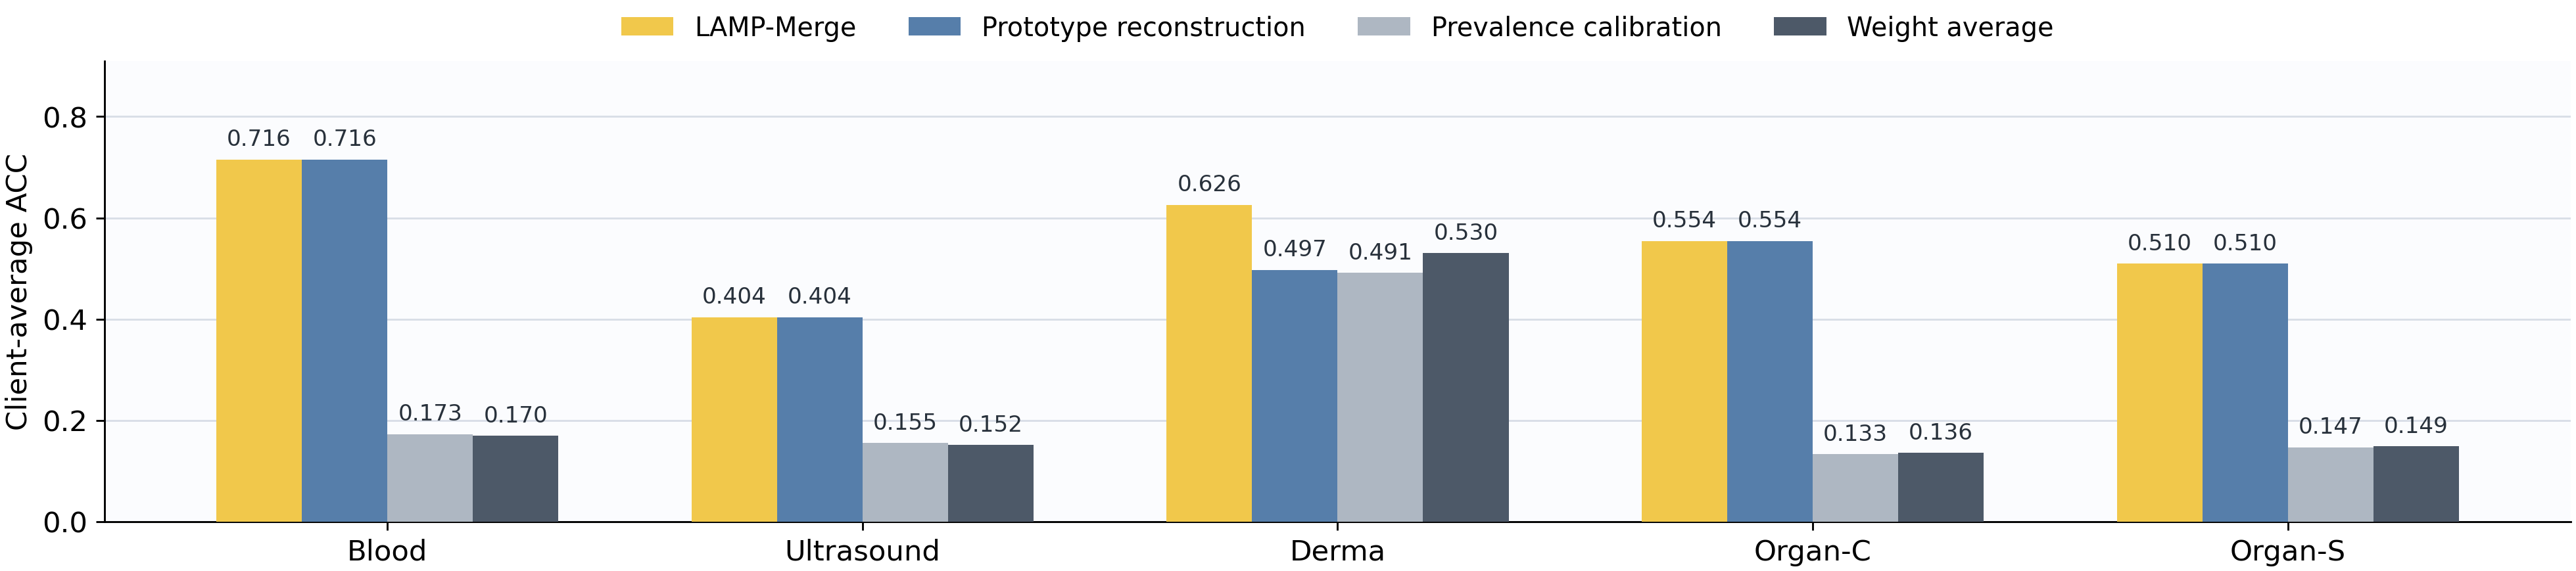
\includegraphics[width=0.92\textwidth]{figures/full_scope_module_ablation_dataset_accuracy.png}
\caption{Dataset-level client-average accuracy in the module ablation. Each dataset contains 12 cells from four vision-model families and three client counts; each cell is averaged over three Dirichlet skew levels.}
\label{fig:dataset-ablation-acc}
\end{figure*}

\subsection{New-metric Diagnostic Experiment}
% 虽然主实验采用 ACC 进行横向比较，但医学长尾分布可能使单类或少数类预测器获得较高 ACC。因此，我们进一步报告平衡准确率、宏 F1、坍缩比例、有效预测类别数以及预测分布与真实分布之间的总变差距离，用于判断准确率提升是否来自更严重的预测坍缩。
Although the main experiments use ACC for direct comparison, long-tailed medical distributions can allow single-class or few-class predictors to achieve high ACC\cite{BUDA2018249,5597285}. We therefore report balanced accuracy, macro-F1, collapse ratio, effective predicted classes, and predicted--true total variation.

\begin{table}[t]
\centering
\caption{Prediction-collapse diagnostics averaged over five medical datasets and four backbones per dataset.}
\label{tab:collapse-key}
\scriptsize
\setlength{\tabcolsep}{3.5pt}
\renewcommand{\arraystretch}{1.35}
\begin{tabular}{lrcc}
\noalign{\hrule height 1.25pt}
\rowcolor[HTML]{F2F2F2}
\textbf{Metric} & \textbf{LAMP-Merge} & \textbf{Best reference} & \textbf{\(\Delta\) vs. reference} \\
\hline \hline
\rowcolor[HTML]{FFF9C4}
\textbf{Accuracy} $\uparrow$ & \textbf{0.6211} & 0.2228 & \compactgain{+39.83\%} \\
BA / macro recall $\uparrow$ & 0.5370 & 0.1492 & \compactgain{+38.78\%} \\
\rowcolor{gray!10}
Macro F1 $\uparrow$ & 0.5238 & 0.0757 & \compactgain{+44.81\%} \\
Collapse ratio $\downarrow$ & 0.3122 & 0.7902 & \compactdrop{-47.80\%} \\
\rowcolor{gray!10}
Effective classes $\uparrow$ & 7.1322 & 2.0489 & \compactgain{+5.0833} \\
Pred-true TV $\downarrow$ & 0.1262 & 0.7040 & \compactdrop{-57.78\%} \\
\noalign{\hrule height 1.25pt}
\end{tabular}
\end{table}

% 表中将 LAMP-Merge 与各个指标上的最佳基线进行比较。结果表明，LAMP-Merge 在准确率之外也显著改善平衡诊断指标和预测分布指标。因此，其准确率提升并非来自更强的单类坍缩，而是来自更完整的全局诊断判别。
Table \ref{tab:collapse-key} compares LAMP-Merge with the best-performing baseline for each metric. \textbf{LAMP-Merge consistently and substantially outperforms the existing methods.} This indicates that its accuracy gains do not arise from more severe single-class prediction collapse, but rather from more complete global diagnostic discrimination.

\subsection{Visualization Experiment}

% 为了直观展示新指标所反映的预测分布变化，我们比较 LAMP-Merge 与最强通用融合方法产生的预测类别分配。通用融合将预测集中到单一主导类别，而 LAMP-Merge 恢复了更广泛、且与测试分布更一致的多类别分配。
To visualize the prediction-distribution changes measured by the new diagnostic metrics, we compare the predicted class allocation induced by LAMP-Merge with that of the strongest generic merge. The generic merge concentrates predictions on one class, whereas LAMP-Merge recovers a broader class allocation aligned with the test distribution.

\begin{figure}[t]
\centering

\includegraphics[width=\linewidth]{figures/full_scope_predicted_distribution_ultrasound_stacked.png}
\caption{Predicted class distributions on Ultrasound, averaged over the four visual backbones, $K\in\{3,5,7\}$, and the three Dirichlet skew levels. The generic merge concentrates predictions on one class, while LAMP-Merge recovers a broader class allocation aligned with the test distribution.}
\label{fig:visual-chaosheng_predict}
\end{figure}

\subsection{Hyperparameter Analysis Experiment}
% 图的上部评估原型头缩放因子 s 和长尾校准强度 lambda。每个取值都在 180 个原始单元和 60 个客户端平均单元上评估，覆盖五个医学数据集、四种骨干网络、三种客户端数量和三种 Dirichlet 非独立同分布划分参数。默认值位于稳定高性能区域，说明收益不是窄范围调参带来的偶然结果。
Fig.~\ref{fig:mechanism-analysis} (top) evaluates the prototype-head scale $s$ and calibration strength $\lambda$ over 180 raw cells and 60 client-average cells. The default $s=20$ and $\lambda=5$ lie in broad stable regions, indicating that the gain is not produced by narrow hyperparameter tuning.

\subsection{t-SNE Visualization Experiment}
% t-SNE 仅用于分析，不参与服务器端选择或融合。图的中部给出 Blood 数据集上 ResNet、K=3、beta=0.01 设置下的联合 t-SNE 对比。每个点对应一个测试图像的输出概率向量，不同融合方法投影到同一二维空间，用于比较预测表征是否形成清晰类别结构。
Fig.~\ref{fig:mechanism-analysis} (middle) uses t-SNE\cite{vanDerMaaten2008} only for analysis on Blood with ResNet, $K=3$, and $\beta=0.01$. LAMP-Merge retains separated output-probability groups, while generic merges exhibit compressed or entangled predictive representations.

\subsection{In-depth Analysis Experiment}
% 最后，我们分析诊断原型重建产生的几何结构。图的下部总结类间分离、最近错误类别间隔、同类客户端一致性以及全局原型与客户端原型对齐程度。结合模块内消融表，该结果说明完整收益来自类别语义原型和类别级支持权重的共同作用，而不是任意分类头带来的表面提升。
Fig.~\ref{fig:mechanism-analysis} (bottom) summarizes inter-class separation, nearest-class margin, within-class client consistency, and prototype--client alignment. Together with Table~\ref{tab:diagnostic-internal-ablation}, the joint profile confirms that class-semantic reference-space prototypes and class-specific support weights provide the mechanism behind the full-scope gain.

\begin{figure*}[!t]
\centering

\includegraphics[width=0.92\textwidth]{figures/full_scope_hyperparameter_sensitivity.png}\par
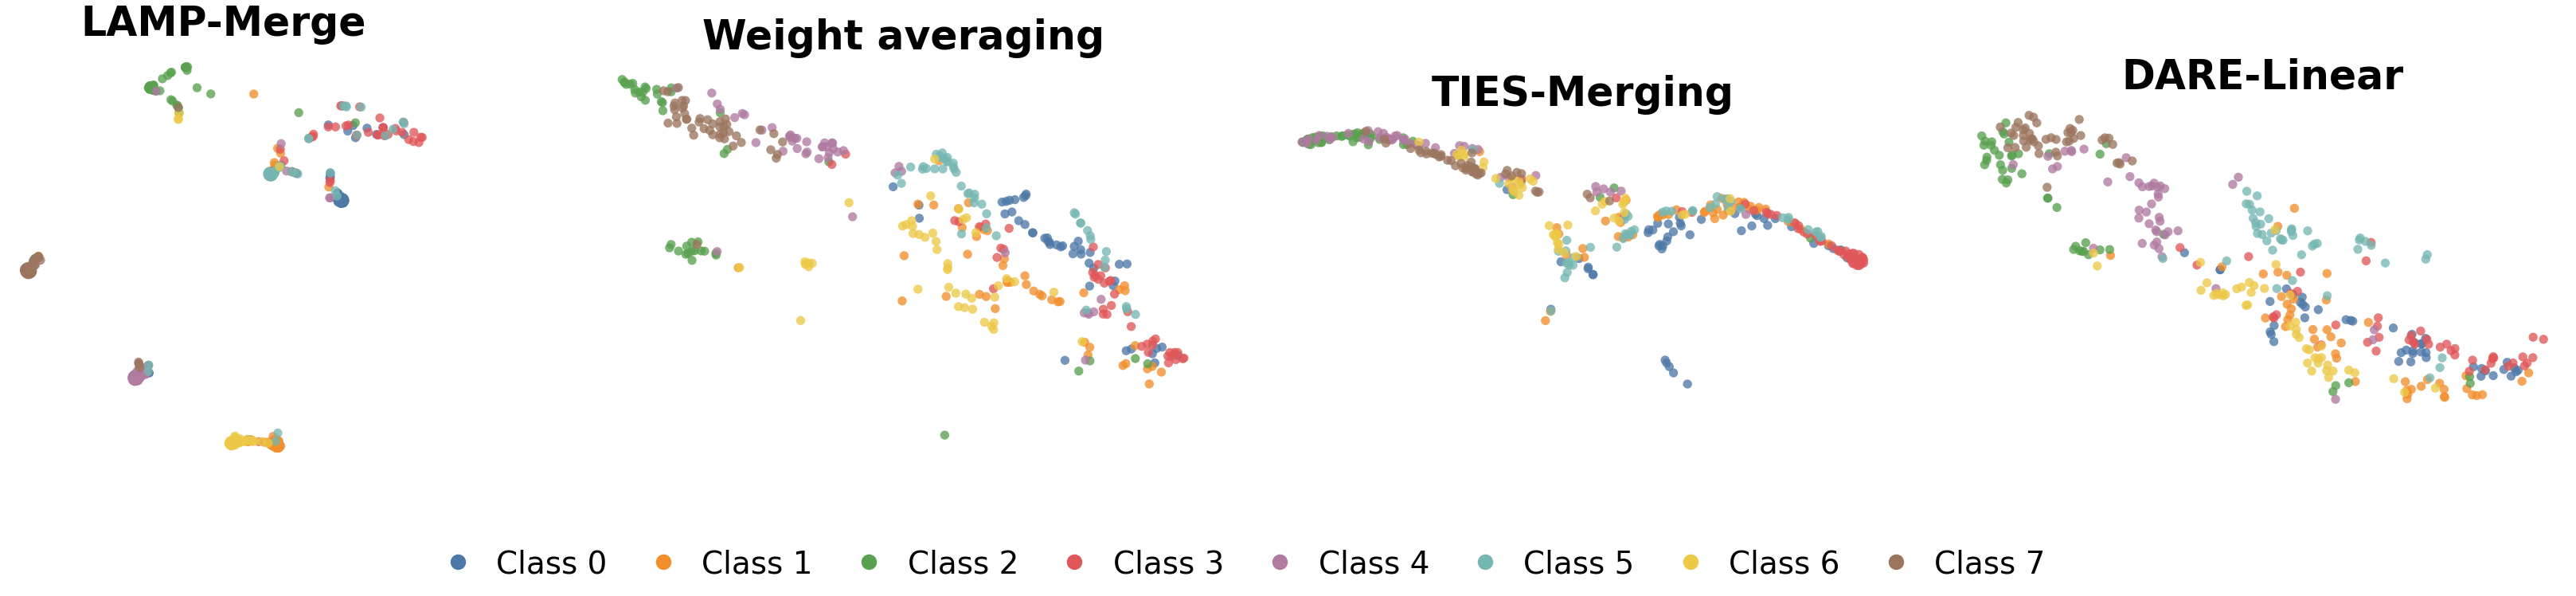
\includegraphics[width=0.98\textwidth]{figures/tsne_joint_bloodmnist_224_resnet.png}\par
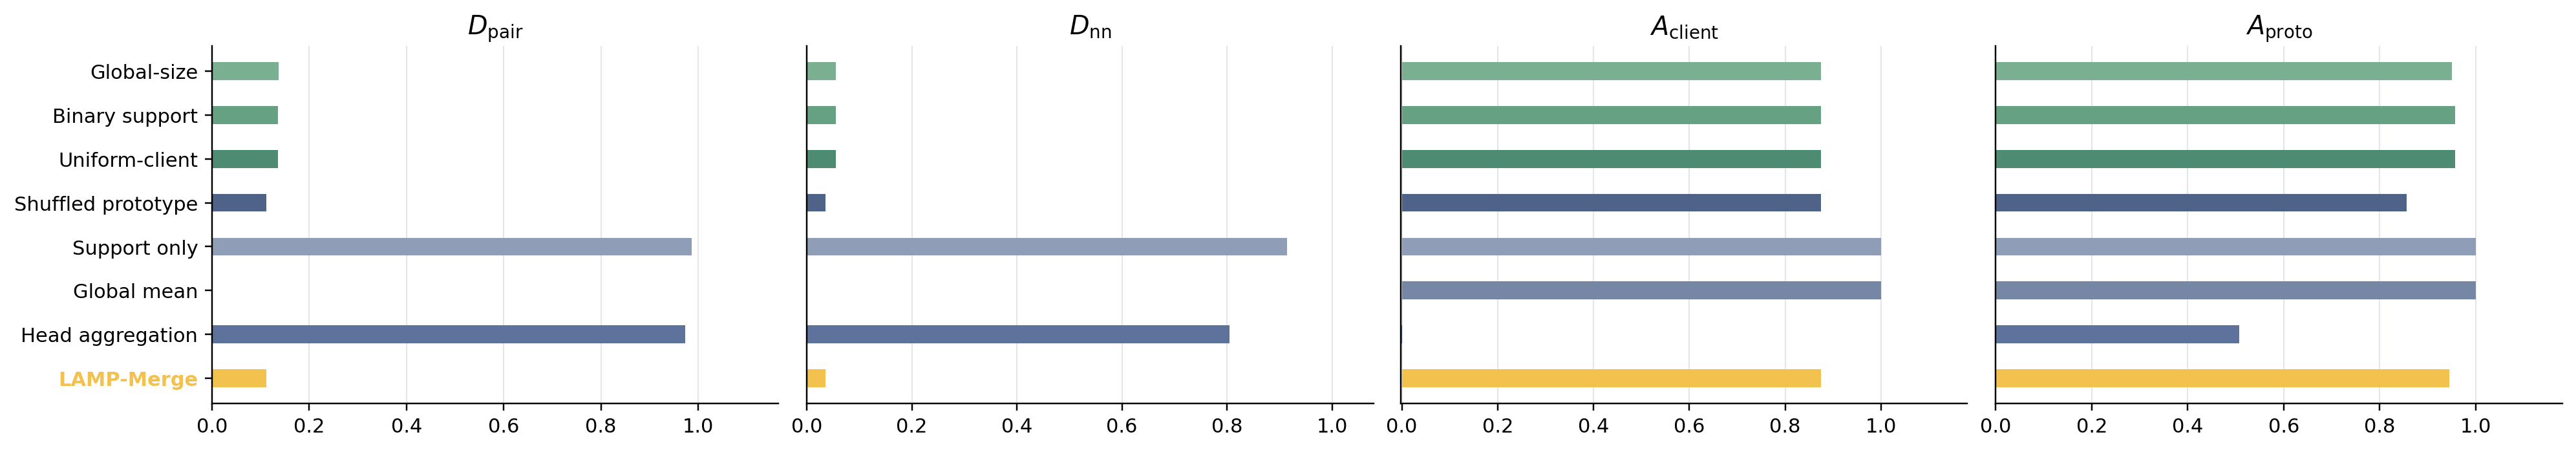
\includegraphics[width=0.96\textwidth]{figures/full_scope_prototype_geometry_internal_ablation.png}
% 顶部：完整范围超参数敏感性；中部：Blood 上的联合 t-SNE；底部：完整基准上的原型几何比较。三组分析共同说明，LAMP-Merge 的提升稳定、能够保持分离的多类别预测，并由类别语义原型几何支撑。
\caption{Core mechanism analyses. Top: full-scope hyperparameter sensitivity, where $s=20$ and $\lambda=5$ lie in stable high-accuracy regions across 180 raw cells and 60 client-average cells. Middle: joint t-SNE of test-image output-probability representations on Blood; from left to right, LAMP-Merge, weight averaging, TIES-Merging, and DARE-Linear. Bottom: full-scope prototype geometry, summarizing pairwise distance, nearest-class distance, prototype consistency, and prototype--client alignment across controlled prototype substitutions. The three panels jointly show that the performance gain is stable, preserves separated multi-class predictions, and is supported by class-semantic prototype geometry rather than an arbitrary classifier head.}
\label{fig:mechanism-analysis}
\end{figure*}

\section{Conclusion}

% 本文重新审视了单次异步医学模型融合问题：独立训练的医院模型必须在没有联邦优化轮次、且不向服务器暴露原始医学图像的条件下完成融合。实证分析表明，当本地诊断覆盖不完整时，通用融合方法会遭遇聚合诱导的预测坍缩。我们进一步指出，在长尾医学数据集上，这种坍缩可能被原始准确率掩盖，因此需要使用宏召回率、宏 F1 和预测分布诊断进行补充评估，并引入长尾患病率校准保留真实患病率结构。
We studied \textbf{one-shot asynchronous medical model merging}, where independently trained hospital models must be fused without federated optimization rounds and without exposing raw medical images to the server. Our empirical analysis shows that generic model-merging methods suffer from \textbf{aggregation-induced predictive collapse} under incomplete local diagnostic coverage. We further show that, on long-tailed medical datasets, such collapse can be masked by raw accuracy. We therefore introduce the Long-tail Prevalence Calibration module and perform secondary evaluation using macro recall, macro-F1, and predictive-distribution diagnostics\cite{BUDA2018249,5597285}.

Taken together, the full-scope comparisons, prediction-distribution diagnostics, and prototype-error analysis establish a consistent mechanism: class-level support-weighted evidence reconstructs discriminative directions for locally absent diagnoses, while bounded prevalence calibration retains clinically meaningful imbalance without reintroducing majority-class collapse.

% LAMP-Merge 通过简洁的双模块设计处理上述两类结构：类别级支持加权证据重建恢复局部缺失诊断的判别方向，有界患病率校准保留临床上有意义的不平衡。未来，我们将从两个方向扩展 LAMP-Merge：一是从医学图像分类推广到分割、检测和多模态诊断任务；二是结合差分隐私或安全聚合等更严格的隐私保护机制，进一步降低类别级统计可能带来的隐私风险。同时，我们也将探索在更大规模真实多中心医疗场景中的部署与验证。
LAMP-Merge addresses these two properties through a concise two-module design. Future work will extend its applicability in two directions: first, from medical image classification to segmentation, detection, and multimodal diagnostic tasks; and second, toward stronger privacy-preserving mechanisms, such as differential privacy and secure aggregation, to further reduce potential privacy risks associated with class-level statistics\cite{kaissis2020secure,geyer2017differentially,abadi2016deep}. We will also explore deployment and validation in larger-scale real-world multicenter healthcare settings.

\bibliography{aaai2026}
\appendix
\section{Supplementary Results and Analysis}

\subsection{Evaluation Datasets}

% \subsubsection{Evaluation Datasets}
% 我们在五个具有代表性的 MedMNIST v2 医学图像基准数据集上评估融合模型。这些数据集覆盖血液显微图像、皮肤镜图像、腹部 CT 器官切片和超声图像等关键医学影像模态，并包含细胞形态识别、皮肤病变诊断、器官结构识别和超声结构判别等任务。
The five MedMNIST v2 benchmarks\cite{yang2023medmnist} cover blood-cell microscopy, dermoscopy, abdominal CT organ slices, and ultrasound images. They involve cell morphology recognition, skin-lesion diagnosis, organ-structure recognition, and ultrasound-structure discrimination:
\begin{itemize}
\item \textbf{Blood}: an eight-class blood-cell microscopy dataset for hematological morphology classification, focusing on fine-grained cellular appearance and inter-class morphological similarity.
\item \textbf{Derma}: a seven-class dermoscopic skin-lesion dataset, characterized by strong long-tailed prevalence and visually subtle lesion categories.
\item \textbf{Organ-C}: an 11-class abdominal CT dataset in the coronal view, evaluating organ-category recognition under grayscale cross-sectional imaging.
\item \textbf{Organ-S}: an 11-class abdominal CT dataset in the sagittal view, complementing Organ-C with a different anatomical imaging plane.
\item \textbf{Ultrasound}: an eight-class ultrasound image dataset, covering structure recognition under modality-specific speckle noise and low-contrast boundaries.
\end{itemize}
% 这些基准数据集构成系统测试平台，用于评估融合模型在不同医学图像类型、不同类别分布和不同成像条件下的跨模态鲁棒性、类别判别能力和任务泛化能力。
Together, these benchmarks provide a systematic testbed for evaluating cross-modality robustness, class-discriminative capability, and task generalization under different medical image types and class-distribution conditions.

\begin{figure*}[t]
\centering
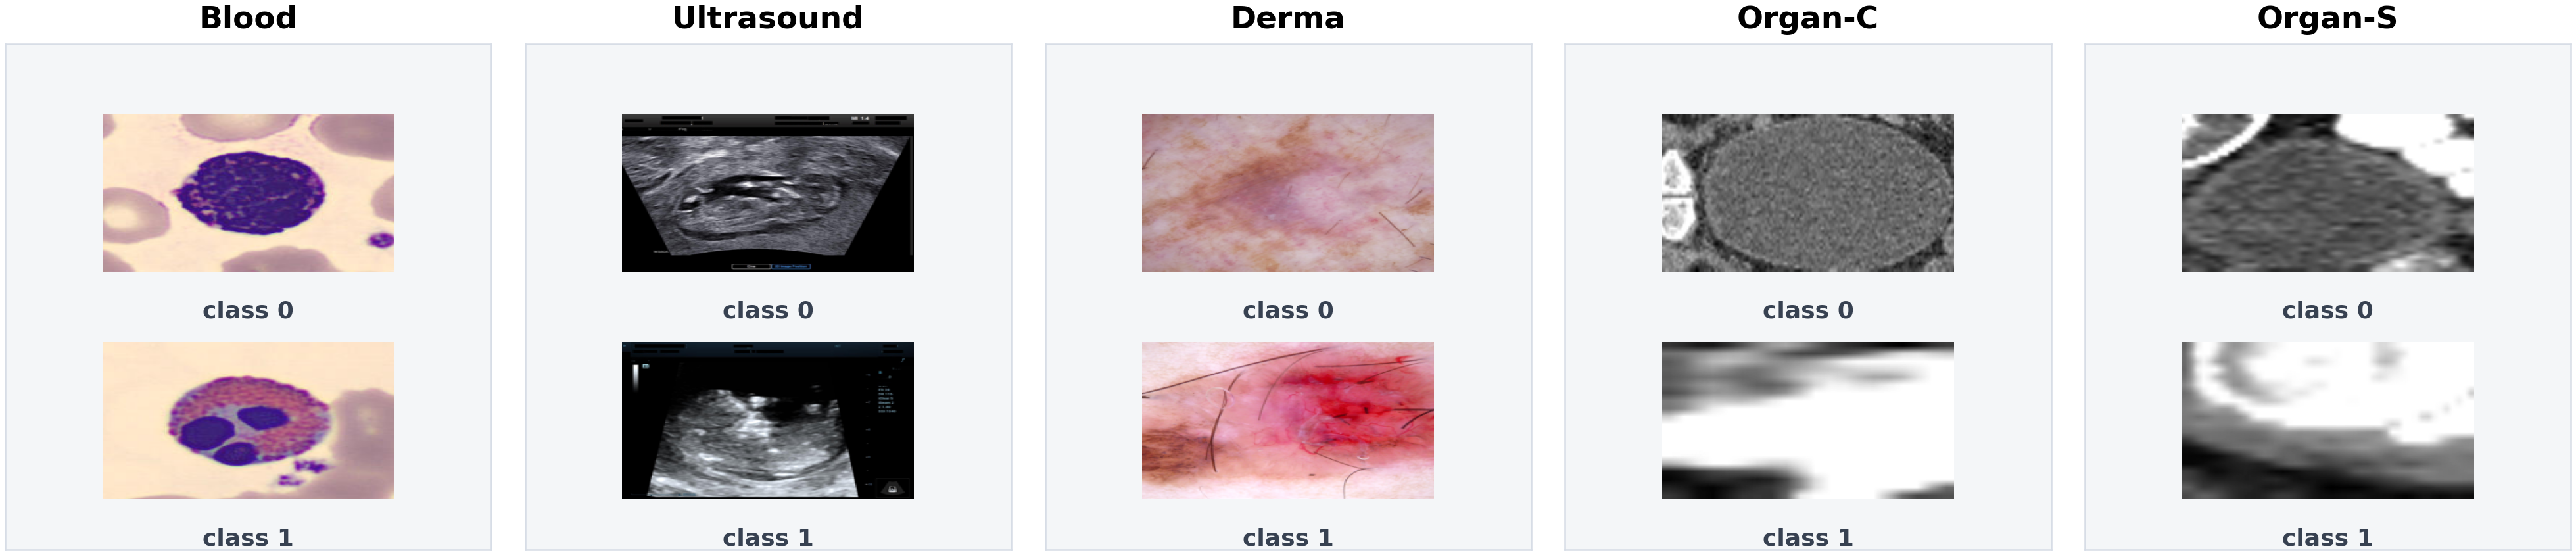
\includegraphics[width=0.96\textwidth]{figures/dataset_examples.png}
\caption{Representative training images from the five medical image datasets used in the experiments. The class IDs are shown only to illustrate category diversity within each dataset.}
\label{fig:dataset-examples}
\end{figure*}

\subsection{Detailed Ablation Configurations}
\label{app:ablation-configurations}

% 诊断原型替换实验均保留长尾患病率校准，只改变原型语义或支持数权重。该设计用于判断收益是否来自参考空间类别原型、类别级支持数，还是仅来自添加一个额外分类头。
All diagnostic-prototype substitutions retain long-tail prevalence calibration and vary only prototype semantics or support-count weighting:
\begin{itemize}
\setlength{\itemsep}{0pt}
\item \textbf{LAMP-Merge} uses \(p_c=\sum_i\alpha_{i,c}\mu_{i,c}\), where \(e_{i,c}=(n_{i,c}+1)^\gamma\mathbf{1}[n_{i,c}>0]\) determines the class-support reliability.
\item \textbf{Classifier-head aggregation} replaces the reference-space class prototype by the local classifier-head direction, i.e., \(\mu_{i,c}\leftarrow h_{i,c}\).
\item \textbf{Global-feature mean} removes class conditioning by setting \(\mu_{i,c}\leftarrow g\) for all \(c\), where \(g\) is the class-agnostic global reference-feature mean.
\item \textbf{Support-only synthetic head} removes image evidence by replacing each prototype with a fixed random unit direction \(u_c\), i.e., \(p_c\leftarrow u_c\), \(\|u_c\|_2=1\).
\item \textbf{Shuffled-label prototype} preserves prototype magnitudes but permutes diagnostic semantics, i.e., \(p_c\leftarrow p_{\sigma(c)}\), where \(\sigma\) is a random permutation over diagnosis labels.
\item \textbf{Uniform client weight} replaces support-weighted aggregation with equal weights among clients containing class \(c\), i.e., \(\alpha_{i,c}\leftarrow \mathbf{1}[n_{i,c}>0]/\sum_j\mathbf{1}[n_{j,c}>0]\).
\item \textbf{Binary support only} replaces fine-grained support and prevalence counts with class-presence indicators, i.e., \(n_{i,c},m_{i,c}\leftarrow \mathbf{1}[n_{i,c}>0]\).
\item \textbf{Global client-size weight} uses the total client support \(N_i=\sum_k n_{i,k}\) rather than class-specific support, i.e., \(e_{i,c}\leftarrow (N_i+1)^\gamma\mathbf{1}[n_{i,c}>0]\).
\end{itemize}

% 长尾患病率替换实验只改变校准偏置中的类别先验，用于判断真实患病率计数是否优于无先验或均匀先验。
The long-tail prevalence substitutions vary only the class prior used by the calibration bias:
\begin{itemize}
\setlength{\itemsep}{0pt}
\item \textbf{LAMP-Merge} estimates the empirical class prior as \(\pi_c=\sum_i m_{i,c}/\sum_k\sum_i m_{i,k}\).
\item \textbf{No prevalence calibration} removes the calibration bias by setting \(b_c\leftarrow0\).
\item \textbf{Uniform prevalence prior} removes long-tail prevalence by setting \(\pi_c\leftarrow 1/C\), where \(C\) is the number of diagnosis classes.
\end{itemize}

\subsubsection{2) Additional Theoretical Analysis}
% 令 mu_c^star 表示共享参考空间中的真实类别均值。如果客户端类别特征具有有界二阶矩，则支持数加权原型的估计误差满足如下上界。
Let $\mu_c^\star$ denote the true class mean in the shared reference space. If client class features have bounded second moments, the prototype estimation error satisfies
\begin{equation}
\mathrm{E}\|p_c-\mu_c^\star\|_2^2
\le
\sum_i \alpha_{i,c}^2\frac{\sigma_c^2}{n_{i,c}}
+ \mathrm{Bias}_c^2.
\end{equation}
% 该上界表明，支持数直接控制类别原型估计方差。没有观测到类别 c 的客户端不应为该类别贡献证据；样本更多的客户端应贡献更多证据，但这种贡献应保持次线性，以避免大客户端完全支配聚合。
This upper bound shows that support counts directly control the variance of class-prototype estimation. A client that does not observe class $c$ should not contribute evidence for that class, and a client with more samples should contribute more, but only sublinearly.

% 令样本 x 在类别 c 和 d 之间的真实间隔为 Delta_c,d(x)。
Let the true margin between classes $c$ and $d$ for sample $x$ be
\begin{equation}
\Delta_{c,d}(x)=(\mu_c^\star)^\top z-(\mu_d^\star)^\top z.
\end{equation}
% 当原型误差小于真实类别间隔所允许的阈值时，估计原型能够保持类别 c 和类别 d 之间的排序。
When the prototype error satisfies
\begin{equation}
\|p_c-\mu_c^\star\|_2+\|p_d-\mu_d^\star\|_2
<
\frac{\Delta_{c,d}(x)}{\|z\|_2},
\end{equation}
the estimated prototypes preserve the class order between $c$ and $d$.

% 长尾患病率校准的作用是以有界方式引入真实长尾先验。对于患病率计数 m_i,c，类别先验为 pi_c，中心化对数先验偏置为 b_c。只要 lambda 有界，长尾校准不会替代诊断原型重建得到的判别方向，而只会将输出校准到真实类别患病率。因此，单独使用长尾校准不足以恢复多类别判别；完整 LAMP-Merge 才能同时保持非坍缩性和患病率感知能力。
The role of long-tail prevalence calibration is to introduce long-tail priors in a bounded manner. For prevalence counts $m_{i,c}$, the class prior is
\begin{equation}
\pi_c=\frac{\sum_i m_{i,c}}{\sum_k \sum_i m_{i,k}},
\end{equation}
and the centered log-prior bias is
\begin{equation}
b_c=\lambda\left(\log\pi_c-\frac{1}{C}\sum_k\log\pi_k\right).
\end{equation}
As long as $\lambda$ is bounded, long-tail prevalence calibration does not replace the discriminative directions reconstructed by diagnostic prototype reconstruction; it only calibrates the output toward the real class prevalence. This explains why using long-tail prevalence calibration alone is insufficient, while full LAMP-Merge remains both non-collapsed and prevalence-aware.

\subsection{Metric Definitions and Geometry Details}
\label{app:metric-geometry}

% 主实验使用 ACC 进行横向比较，但医学长尾分布可能使单类或少数类预测器获得较高 ACC。因此，我们定义预测分布诊断指标。令 y_n 和 \hat y_n 分别表示第 n 个测试样本的真实标签和预测标签，q_c 表示预测类别分布，p_c 表示真实类别分布，C_test 表示测试集中真实出现的类别集合。
Let \(y_n\) and \(\hat{y}_n\) denote the true and predicted labels of the \(n\)-th test sample. Let \(q_c=N^{-1}\sum_n\mathbf{1}[\hat{y}_n=c]\) be the predicted-class distribution, \(p_c=N^{-1}\sum_n\mathbf{1}[y_n=c]\) the true class distribution, and \(\mathcal{C}_{\mathrm{test}}=\{c\mid \sum_n\mathbf{1}[y_n=c]>0\}\) the set of classes observed in the test set. We use:
\begin{itemize}
\setlength{\itemsep}{0pt}
\item \(\mathrm{BA}=|\mathcal{C}_{\mathrm{test}}|^{-1}\sum_{c\in\mathcal{C}_{\mathrm{test}}}\mathrm{Recall}_c\), balanced accuracy or macro recall, which measures whether all observed diagnosis classes are recalled.
\item \(\mathrm{MacroF1}=|\mathcal{C}_{\mathrm{test}}|^{-1}\sum_{c\in\mathcal{C}_{\mathrm{test}}}\mathrm{F1}_c\), class-balanced precision-recall quality that penalizes majority-only predictions.
\item \(\rho=\max_c q_c\), the prediction-collapse ratio, which measures concentration on a single diagnosis class.
\item \(C_{\mathrm{eff}}=\exp\left(-\sum_c q_c\log q_c\right)\), the effective number of predicted classes.
\item \(\mathrm{TV}(q,p)=\frac{1}{2}\sum_c |q_c-p_c|\), the total variation distance between predicted and true class distributions.
\end{itemize}

% 最后，我们定义原型几何指标，用于解释诊断原型重建为什么有效。该分析对应模块内消融中的原型替换设置，重点观察参考空间类别原型是否形成稳定的类间分离、最近类间隔、客户端一致性和全局-本地原型对齐。令 d(a,b)=1-cos(a,b) 表示余弦距离，I_c 表示具有类别 c 样本的客户端集合。
Let \(d(a,b)=1-\cos(a,b)\) denote cosine distance and let \(\mathcal{I}_c=\{i\mid n_{i,c}>0\}\) denote the clients that contain diagnosis class \(c\). The geometric quantities are:
\begin{itemize}
\setlength{\itemsep}{0pt}
\item \(D_{\mathrm{pair}}=\frac{2}{C(C-1)}\sum_{c<d}d(p_c,p_d)\), the mean distance between global prototypes of different diagnosis classes.
\item \(D_{\mathrm{nn}}=\frac{1}{C}\sum_c \min_{d\ne c} d(p_c,p_d)\), the mean nearest-class distance and most vulnerable decision margin.
\item \(A_{\mathrm{client}}=\frac{1}{C}\sum_c \mathrm{Avg}_{i<j,\,i,j\in\mathcal{I}_c}\cos(\mu_{i,c},\mu_{j,c})\), the within-class consistency among client prototypes; \(A_{\mathrm{proto}}=\frac{1}{C}\sum_c\sum_{i\in\mathcal{I}_c}\alpha_{i,c}\cos(p_c,\mu_{i,c})\), the alignment between the global prototype and contributing client prototypes.
\end{itemize}

\end{document}
